% Compile from the project root with:
% pdflatex -output-directory=reports reports/presentation.tex

\documentclass[10pt,aspectratio=169]{beamer}

\usepackage[utf8]{inputenc}
\usepackage[T1]{fontenc}
\usepackage{lmodern}
\usepackage{booktabs}
\usepackage{graphicx}
\usepackage{array}
\usepackage{xcolor}
\usepackage{amsmath}

\usetheme{Madrid}
\usecolortheme{default}
\setbeamertemplate{navigation symbols}{}
\setbeamertemplate{footline}[frame number]

\definecolor{oodblue}{RGB}{25,77,132}
\definecolor{oodteal}{RGB}{0,125,132}
\definecolor{oodorange}{RGB}{199,100,31}
\setbeamercolor{structure}{fg=oodblue}
\setbeamercolor{frametitle}{fg=white,bg=oodblue}
\setbeamercolor{title}{fg=white,bg=oodblue}

\graphicspath{
  {results/figures/}
  {results/roc_curves/}
  {results/score_distributions/}
  {results/tsne_umap/}
  {results/confusion_matrices/}
  {../results/figures/}
  {../results/roc_curves/}
  {../results/score_distributions/}
  {../results/tsne_umap/}
  {../results/confusion_matrices/}
}

\title[OOD Detection in Computer Vision]{Out-of-Distribution Detection in Computer Vision}
\subtitle{Comparative benchmark with a simplified STOOD-X statistical approach}
\author{Leonel Silima \and Luís Lucas}
\institute{Computer Vision -- PDEEC \quad FEUP, University of Porto}
\date{Academic Year 2025/2026}

\begin{document}

\begin{frame}
  \titlepage
\end{frame}

\begin{frame}{Problem and Objective}
  \begin{columns}[T,onlytextwidth]
    \column{0.58\textwidth}
      \textbf{Problem.} A classifier trained on CIFAR-10 can still assign high confidence to images outside its training distribution.

      \vspace{0.6em}
      \textbf{Objective.} Detect whether an input image is In-Distribution (ID) or Out-of-Distribution (OOD), while keeping the trained classifier fixed.

      \vspace{0.6em}
      \textbf{Project focus.}
      \begin{itemize}
        \item Train ResNet-18 on CIFAR-10.
        \item Benchmark post-hoc OOD detectors.
        \item Partially replicate the feature-space intuition of STOOD-X.
      \end{itemize}
    \column{0.38\textwidth}
      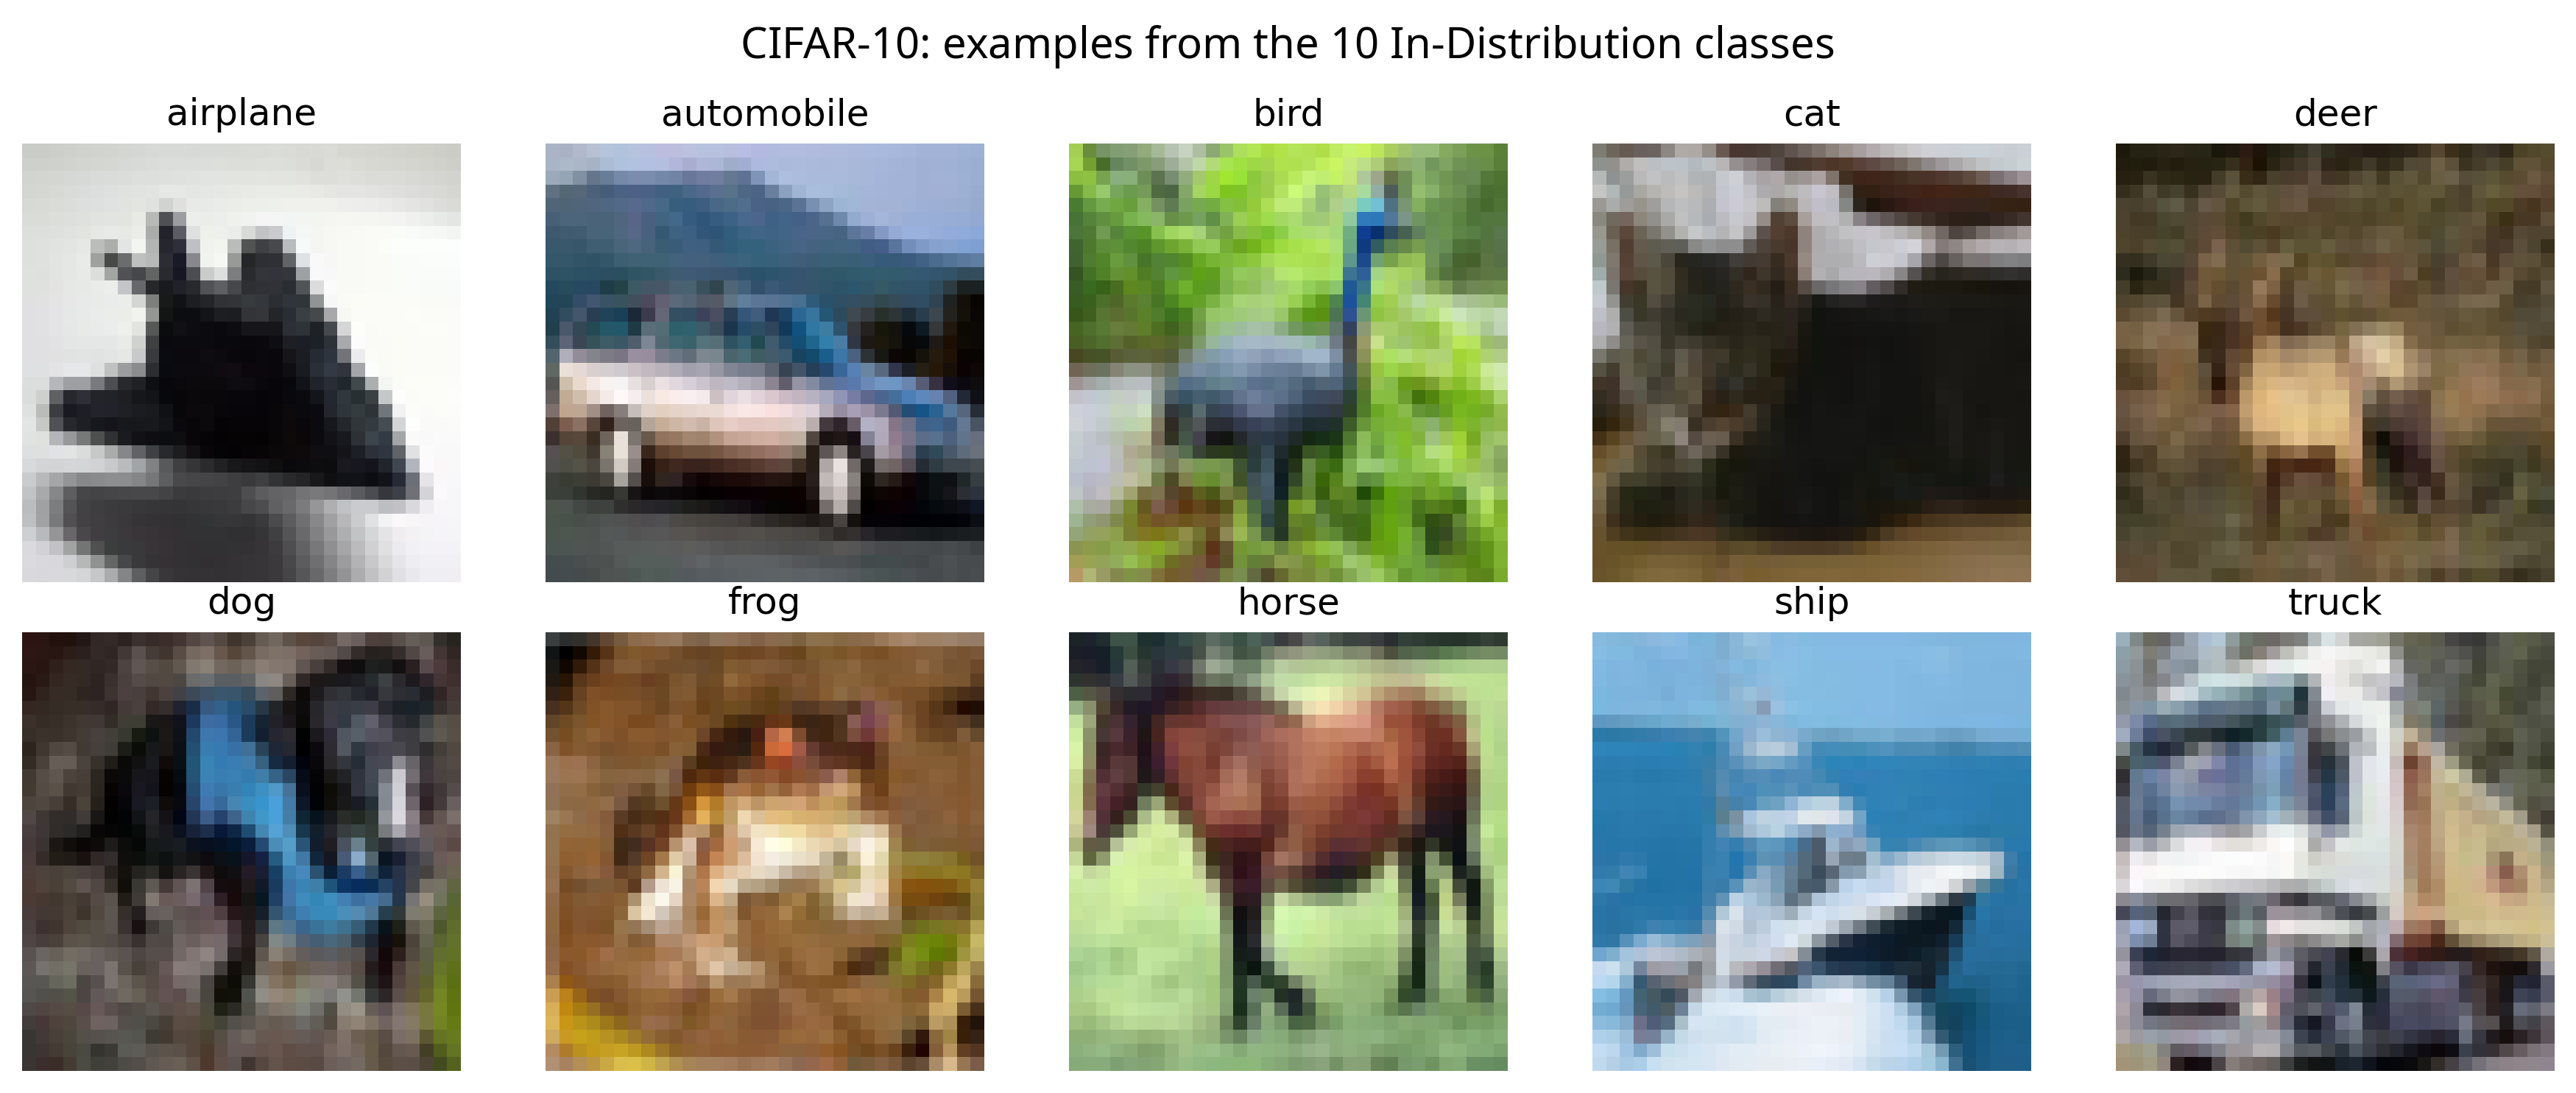
\includegraphics[width=\textwidth]{cifar10_examples_grid.png}
      \vspace{0.3em}

      \centering{\small CIFAR-10 is the known distribution.}
  \end{columns}
\end{frame}

\begin{frame}{Experimental Setup}
  \begin{columns}[T,onlytextwidth]
    \column{0.46\textwidth}
      \textbf{Datasets}
      \begin{itemize}
        \item ID: CIFAR-10.
        \item OOD: CIFAR-100, SVHN, MNIST.
        \item All inputs normalized with CIFAR-10 statistics.
      \end{itemize}

      \vspace{0.4em}
      \textbf{Classifier}
      \begin{itemize}
        \item ResNet-18 adapted for $32\times32$ images.
        \item 20 training epochs.
        \item Best CIFAR-10 test accuracy: \textbf{91.03\%}.
      \end{itemize}
    \column{0.50\textwidth}
      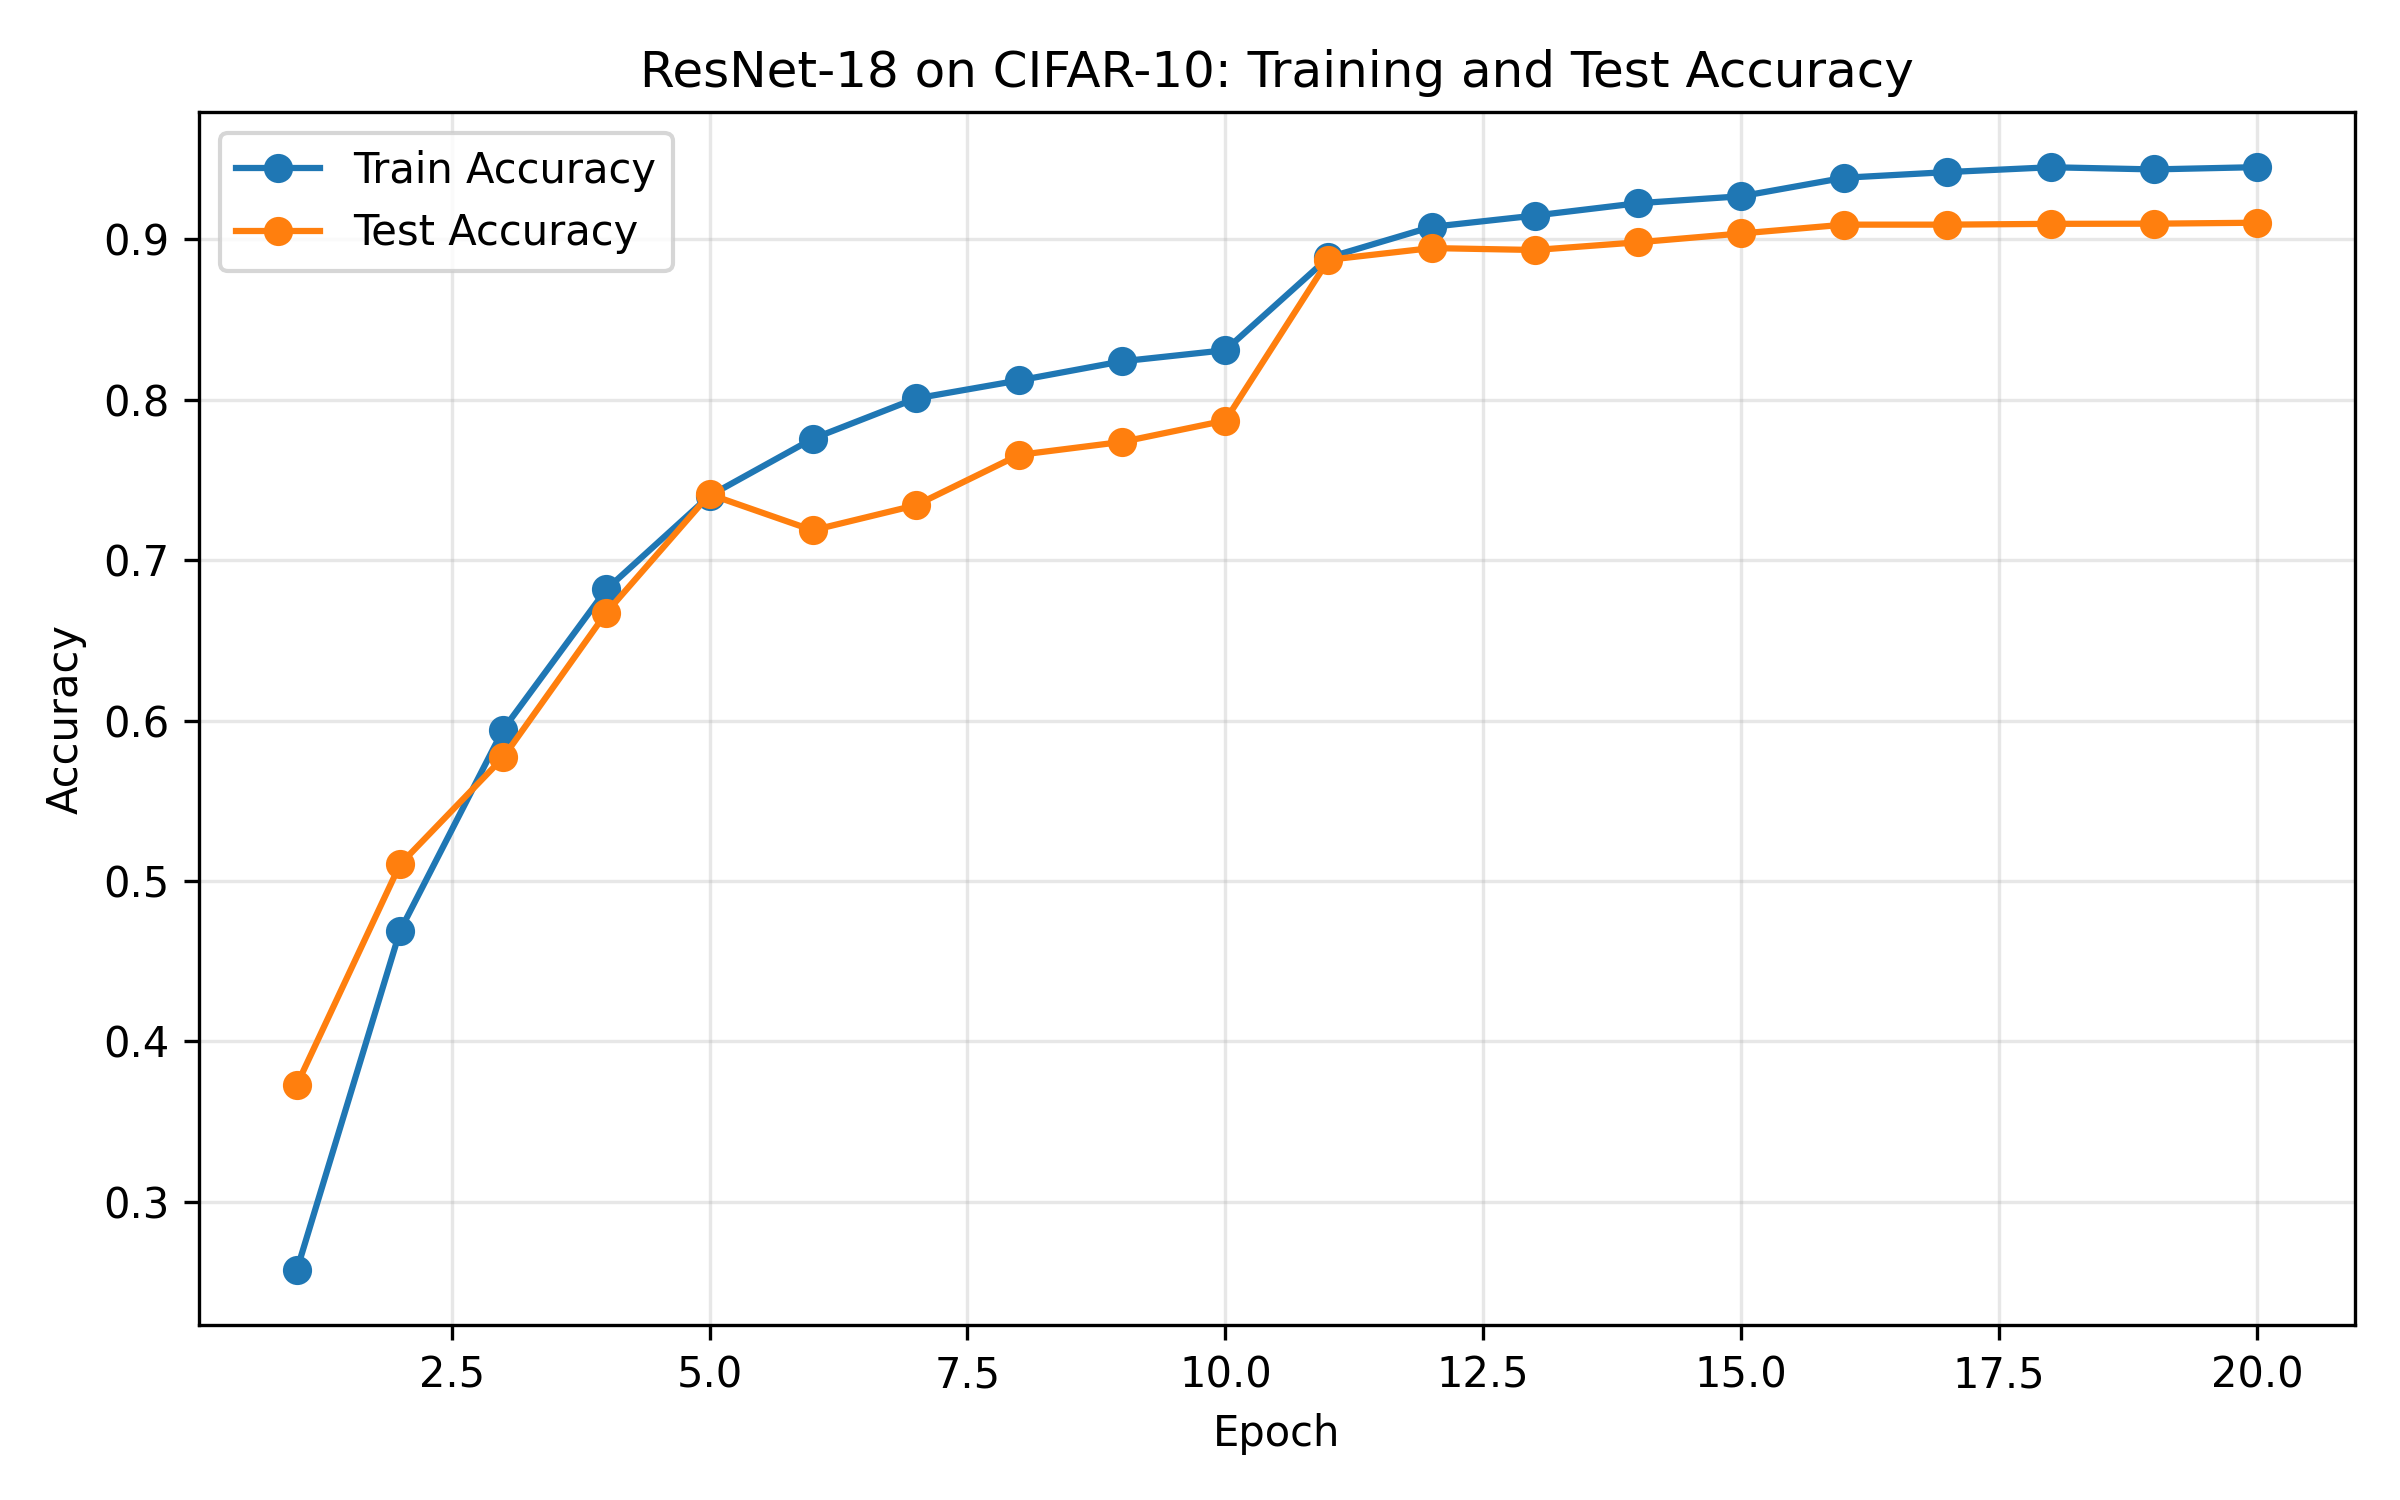
\includegraphics[width=0.49\textwidth]{training_accuracy_resnet18_cifar10.png}
      \hfill
      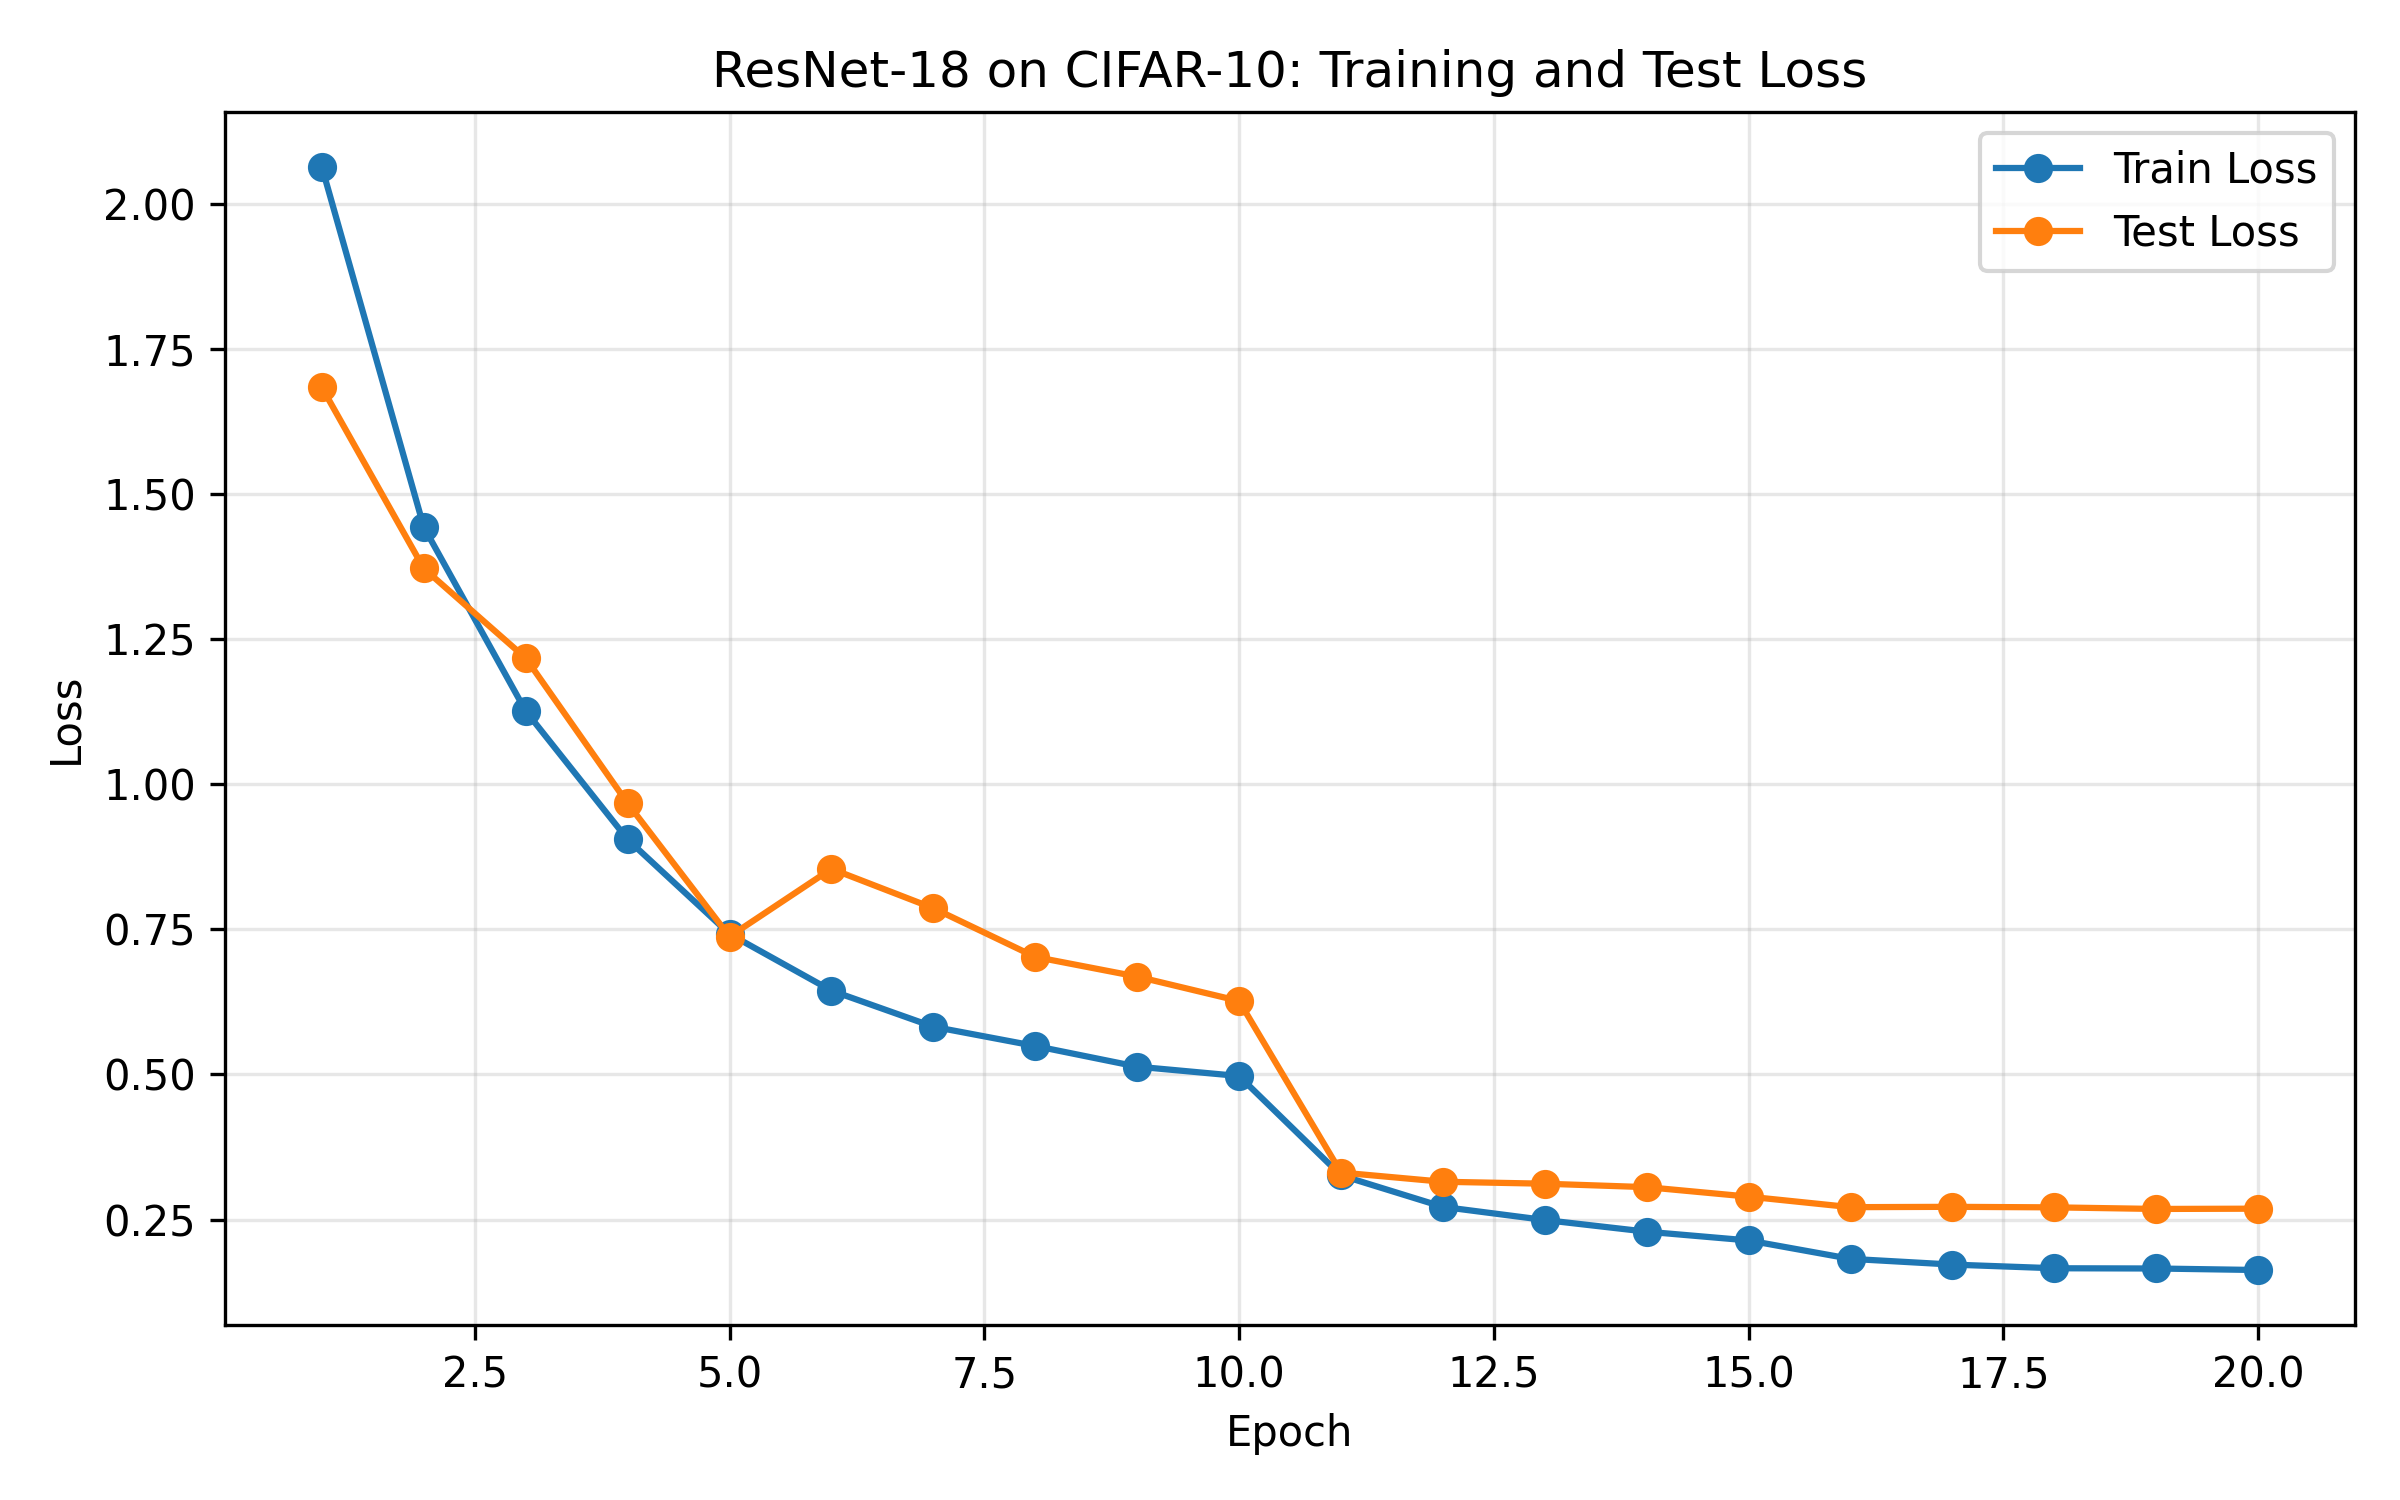
\includegraphics[width=0.49\textwidth]{training_loss_resnet18_cifar10.png}

      \vspace{0.7em}
      \textbf{Metrics}
      \begin{itemize}
        \item AUROC, AUPR-IN, AUPR-OUT: higher is better.
        \item FPR95: lower is better.
      \end{itemize}
  \end{columns}
\end{frame}

\begin{frame}{Methods Compared}
  \begin{columns}[T,onlytextwidth]
    \column{0.48\textwidth}
      \textbf{Logit/confidence based}
      \begin{itemize}
        \item \textbf{MSP}: maximum softmax probability.
        \item \textbf{Energy}: log-sum-exp score over logits.
        \item \textbf{ODIN}: temperature scaling plus input perturbation.
      \end{itemize}

      \vspace{0.8em}
      These methods use the classifier output directly.
    \column{0.48\textwidth}
      \textbf{Feature-distance based}
      \begin{itemize}
        \item \textbf{Mahalanobis}: distance to class feature means.
        \item \textbf{KNN}: distance to the ID feature bank, $k=50$.
        \item \textbf{STOOD-X simplified}: empirical p-value from KNN distances.
      \end{itemize}

      \vspace{0.8em}
      These methods use penultimate-layer representations.
  \end{columns}

  \vspace{0.7em}
  \centering
  \textbf{Common convention:} high score = more likely ID; low score = more likely OOD.
\end{frame}

\begin{frame}{Simplified STOOD-X Procedure}
  \begin{columns}[T,onlytextwidth]
    \column{0.55\textwidth}
      \begin{enumerate}
        \item Extract ResNet-18 features from CIFAR-10 training images.
        \item Build an ID feature bank.
        \item For each ID training sample, compute the distance to its $k$-th nearest neighbor.
        \item Use these distances as the reference ID distribution.
        \item For a new sample, convert its KNN distance into an empirical p-value.
      \end{enumerate}
    \column{0.40\textwidth}
      \[
      p(x)=\frac{1}{N}\sum_{i=1}^{N}
      \mathbb{I}\left(d_i^{ref}\geq d(x)\right)
      \]

      \vspace{1.0em}
      \textbf{Interpretation}
      \begin{itemize}
        \item High p-value: close to ID feature geometry.
        \item Low p-value: statistically unusual feature distance.
      \end{itemize}
  \end{columns}

  \vspace{0.5em}
  \small This is a partial replication: the full STOOD-X explainability stage and the original Wilcoxon-Mann-Whitney test were not implemented.
\end{frame}

\begin{frame}{Quantitative Benchmark}
  \centering
  \small
  \begin{tabular}{llcc}
    \toprule
    OOD Dataset & Best AUROC & Best FPR95 & Strongest Pattern \\
    \midrule
    CIFAR-100 & ODIN: \textbf{0.8810} & Energy: \textbf{0.5825} & hardest near-OOD case \\
    MNIST & ODIN: \textbf{0.9643} & Energy: \textbf{0.2073} & easiest far-OOD case \\
    SVHN & STOOD-X: \textbf{0.9339} & STOOD-X: \textbf{0.4916} & feature distances win \\
    \bottomrule
  \end{tabular}

  \vspace{1.0em}
  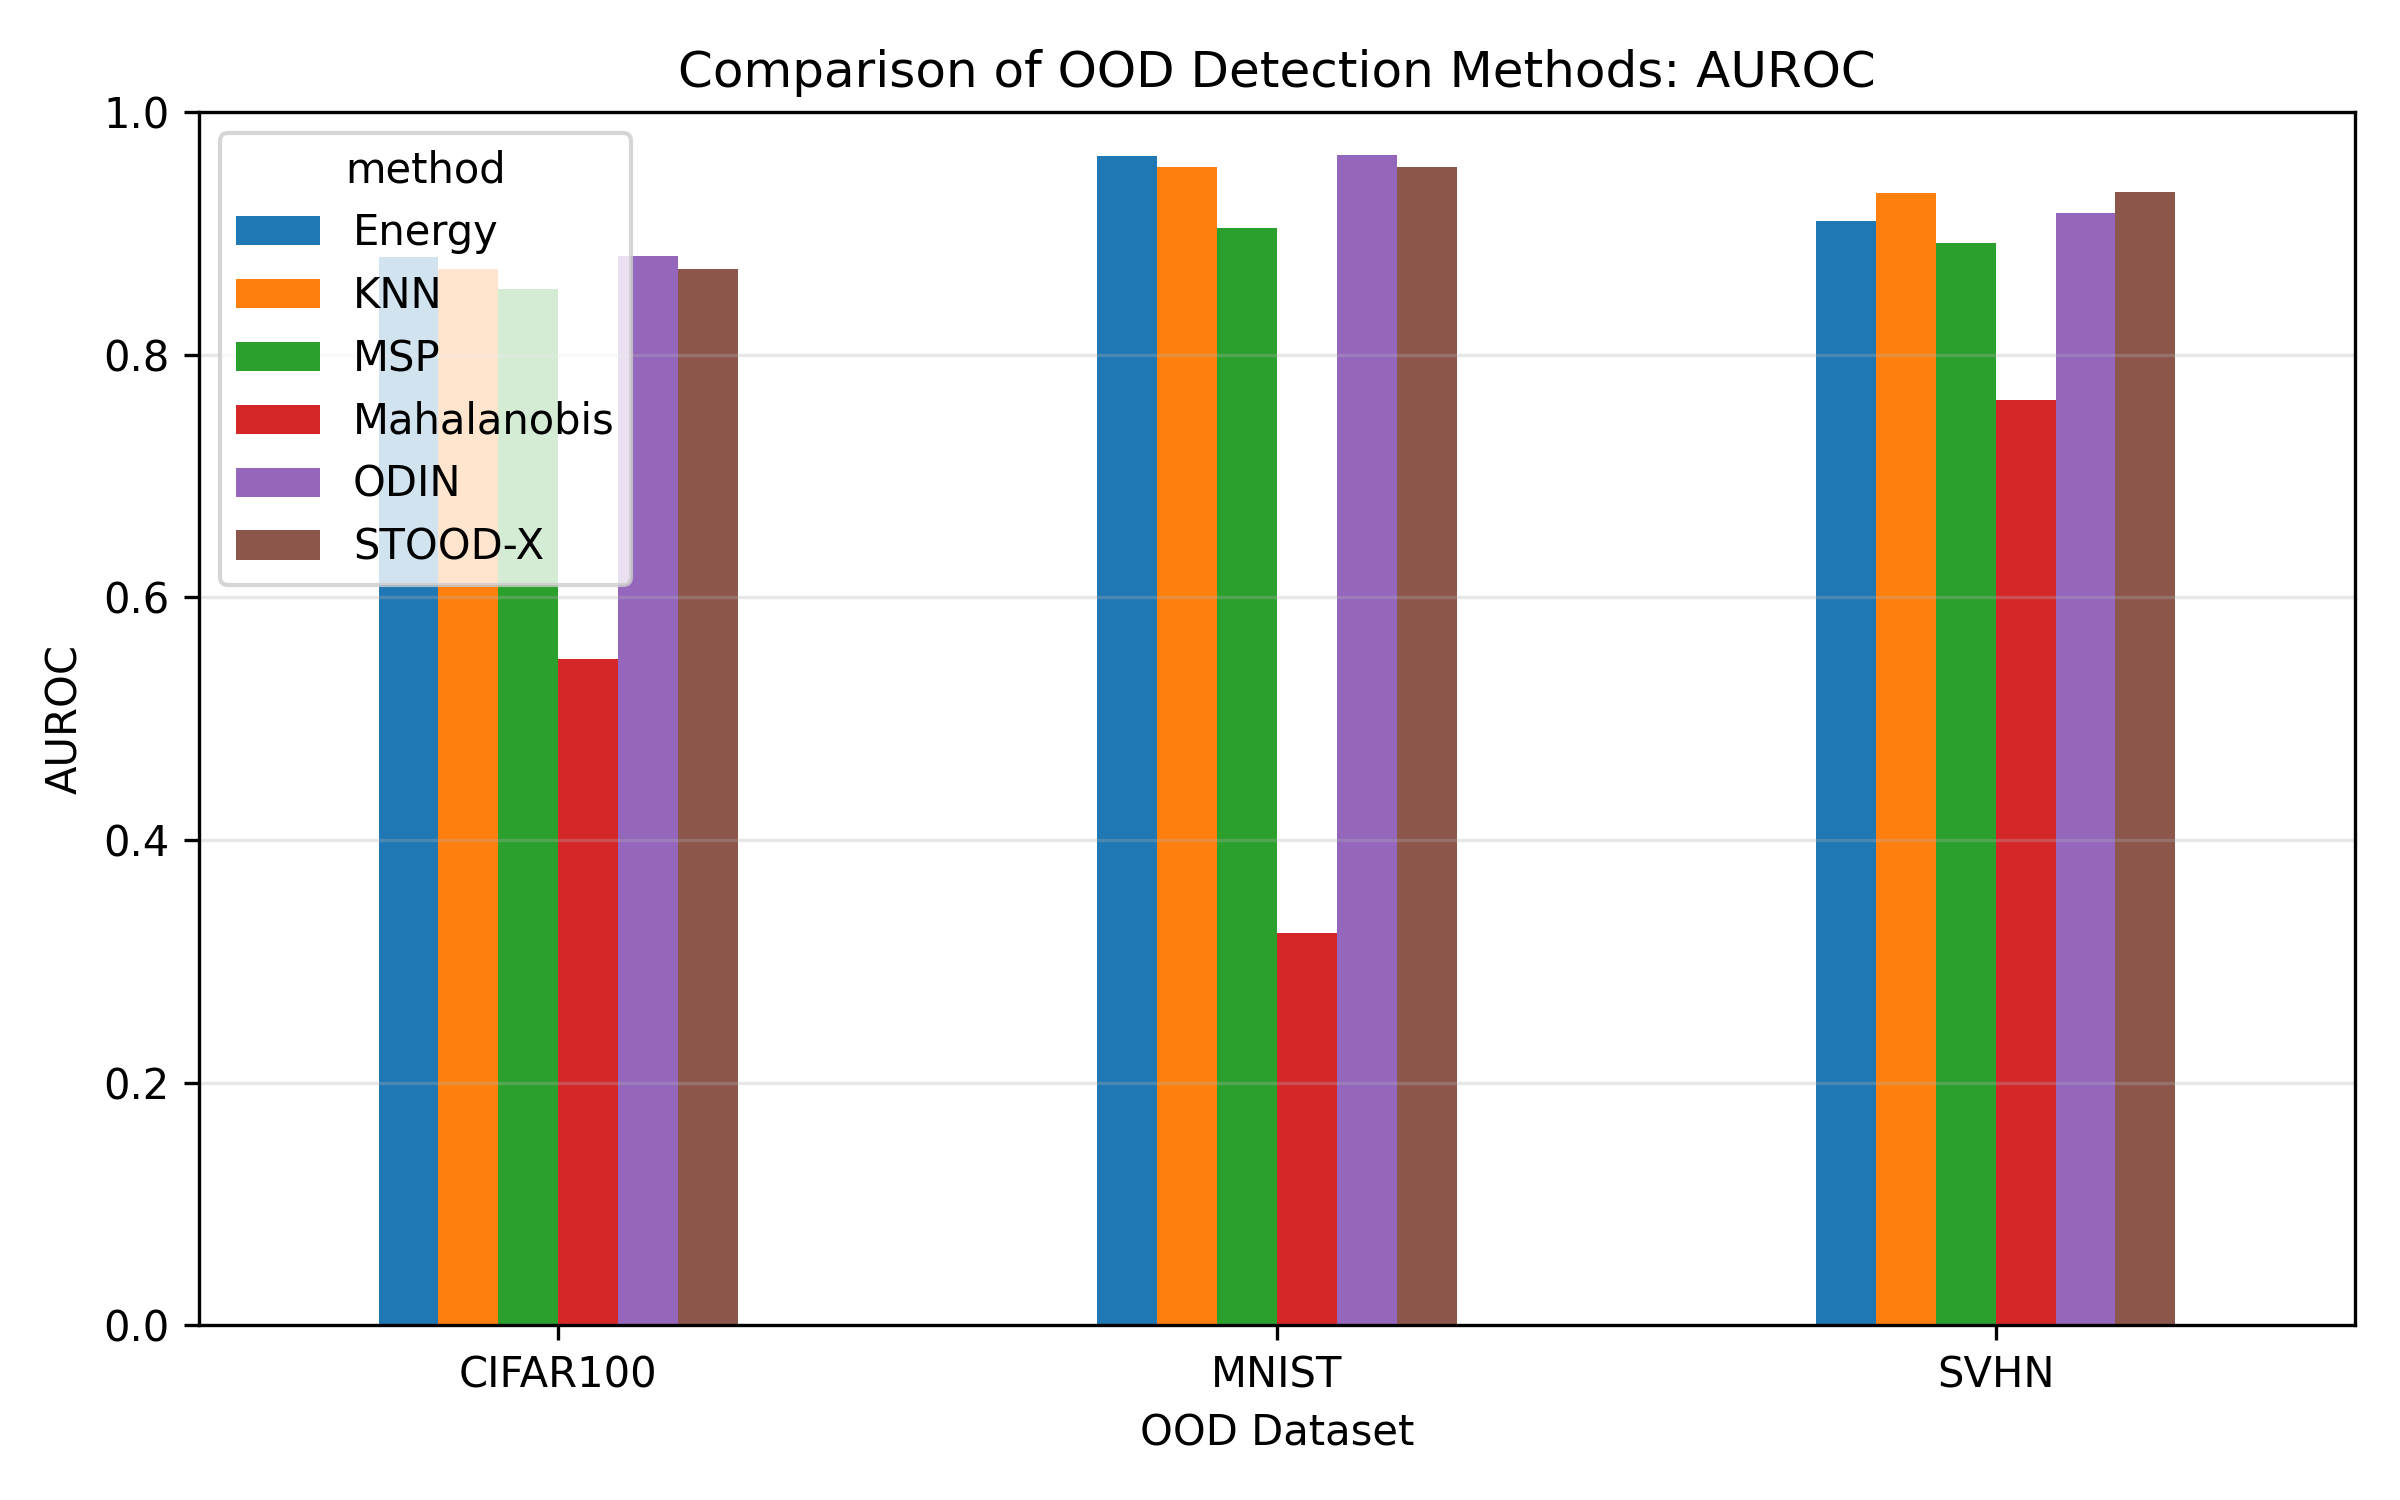
\includegraphics[width=0.47\textwidth]{comparison_methods_auroc.png}
  \hfill
  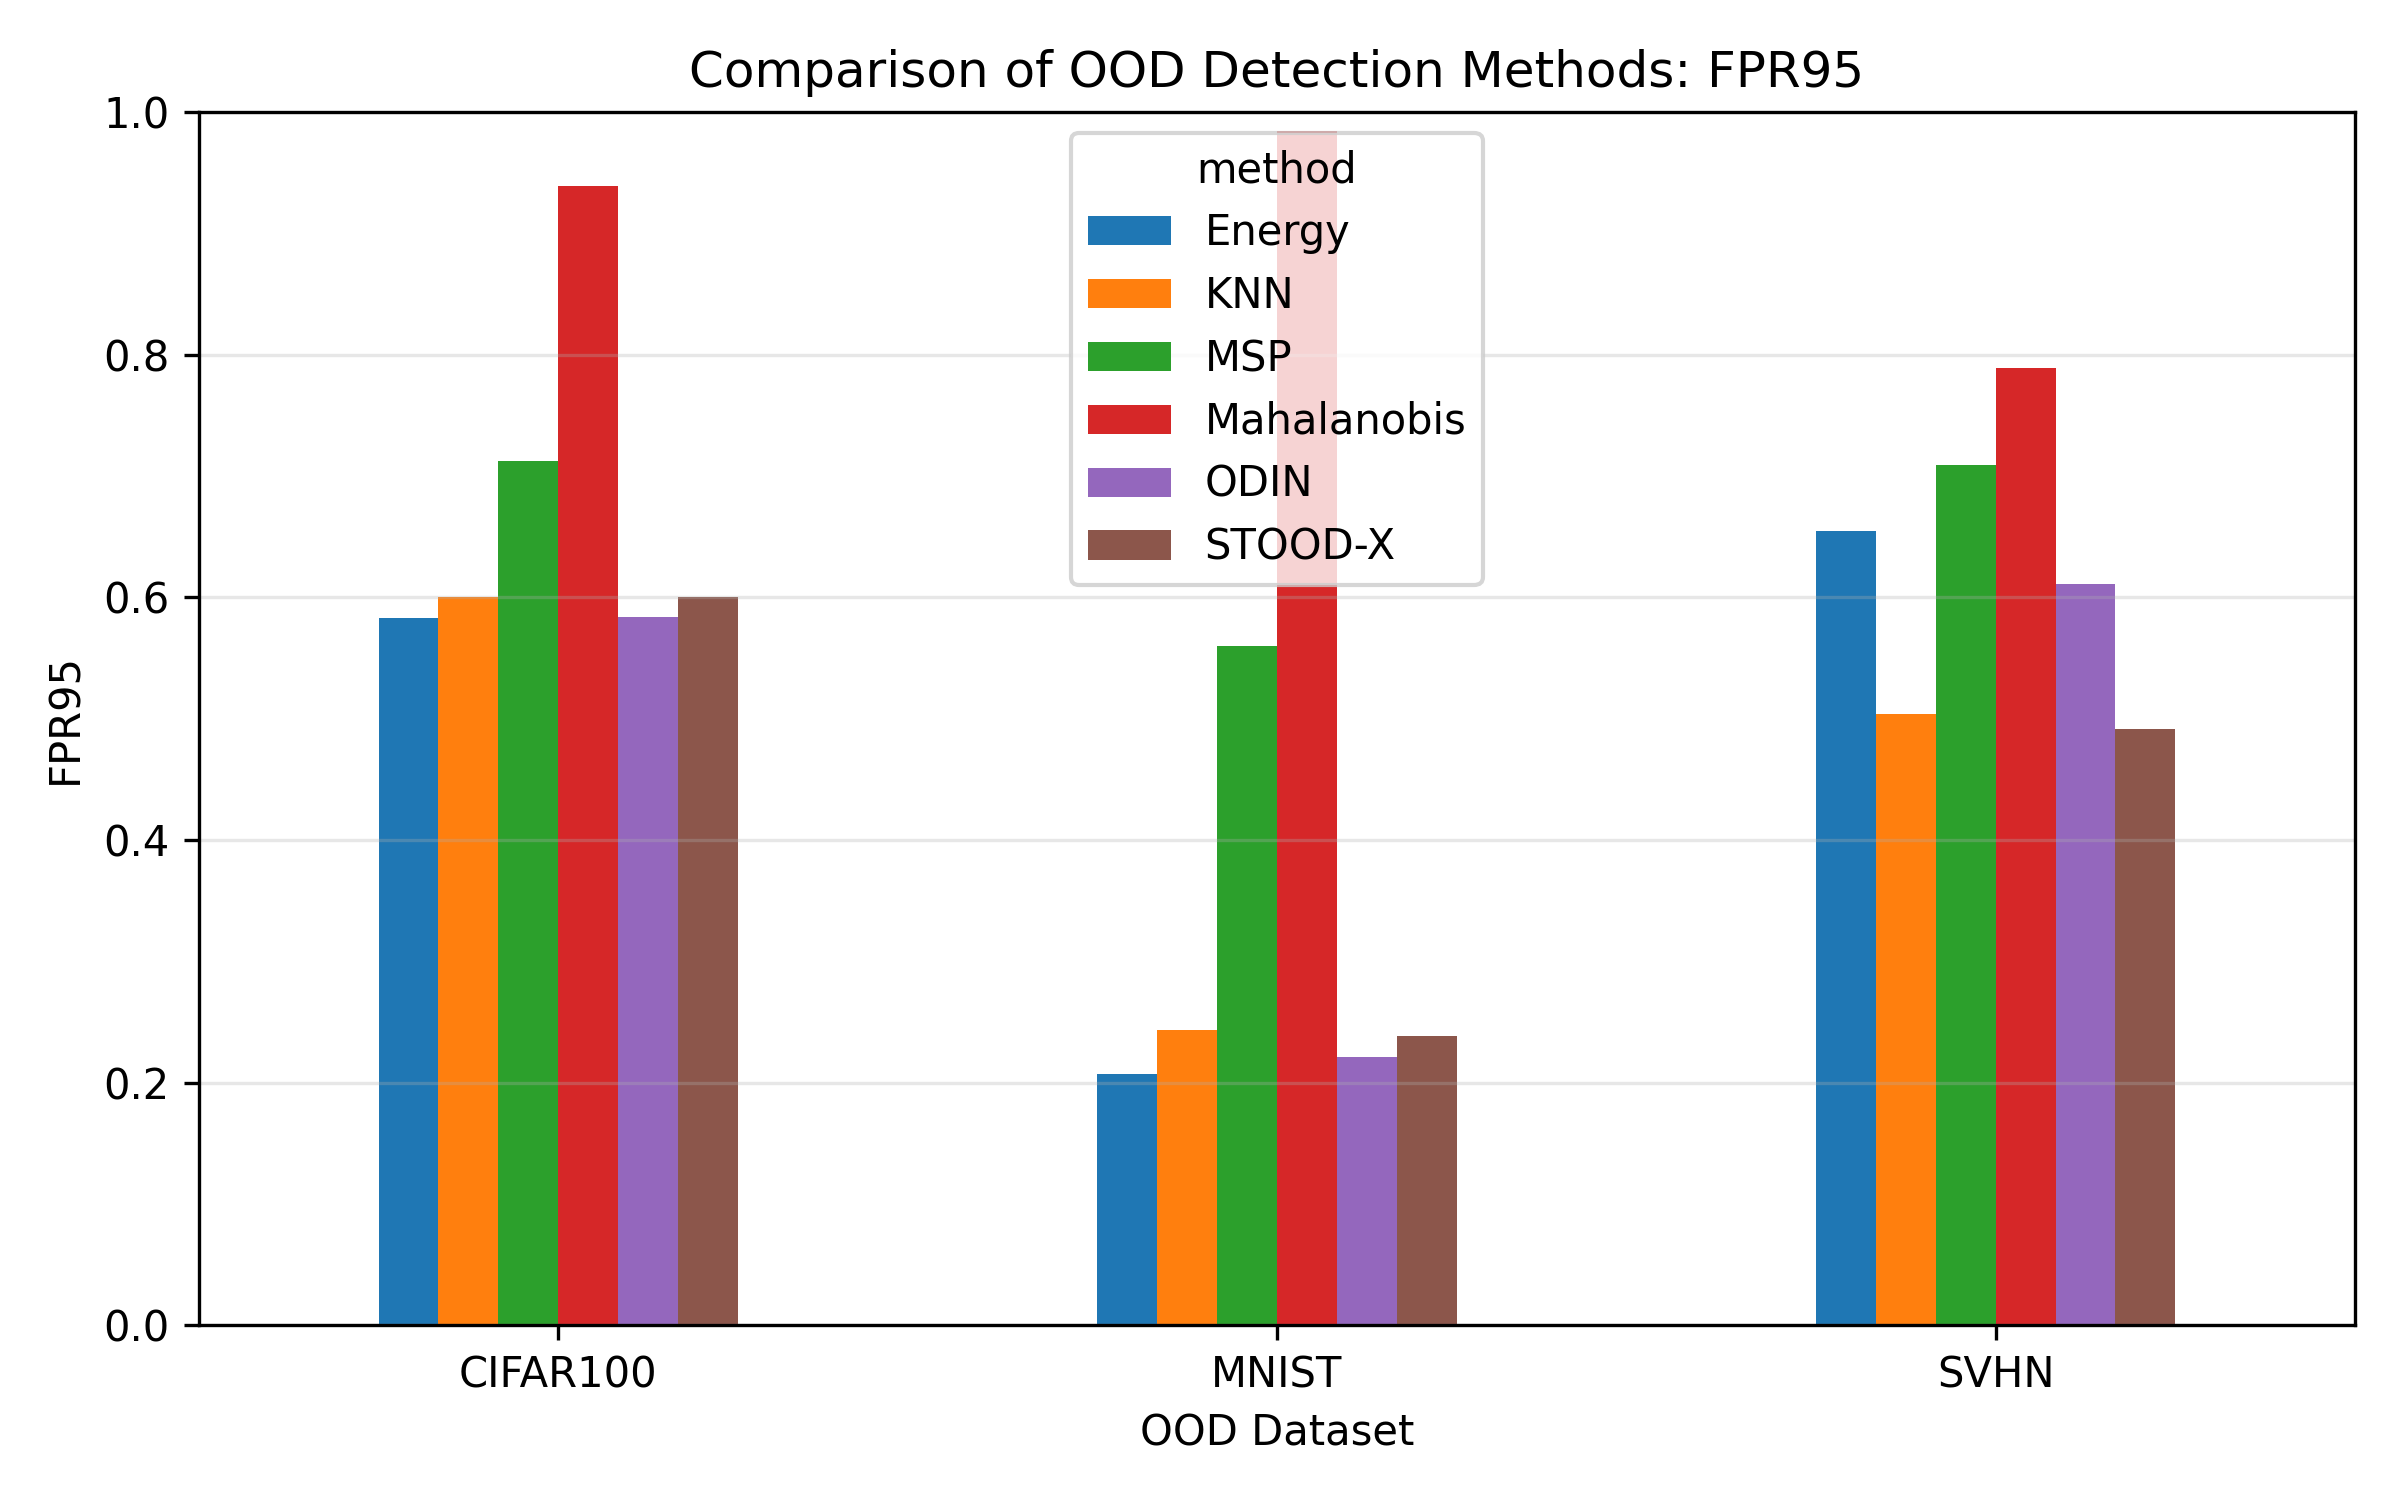
\includegraphics[width=0.47\textwidth]{comparison_methods_fpr95.png}
\end{frame}

\begin{frame}{Full Result Matrix}
  \centering
  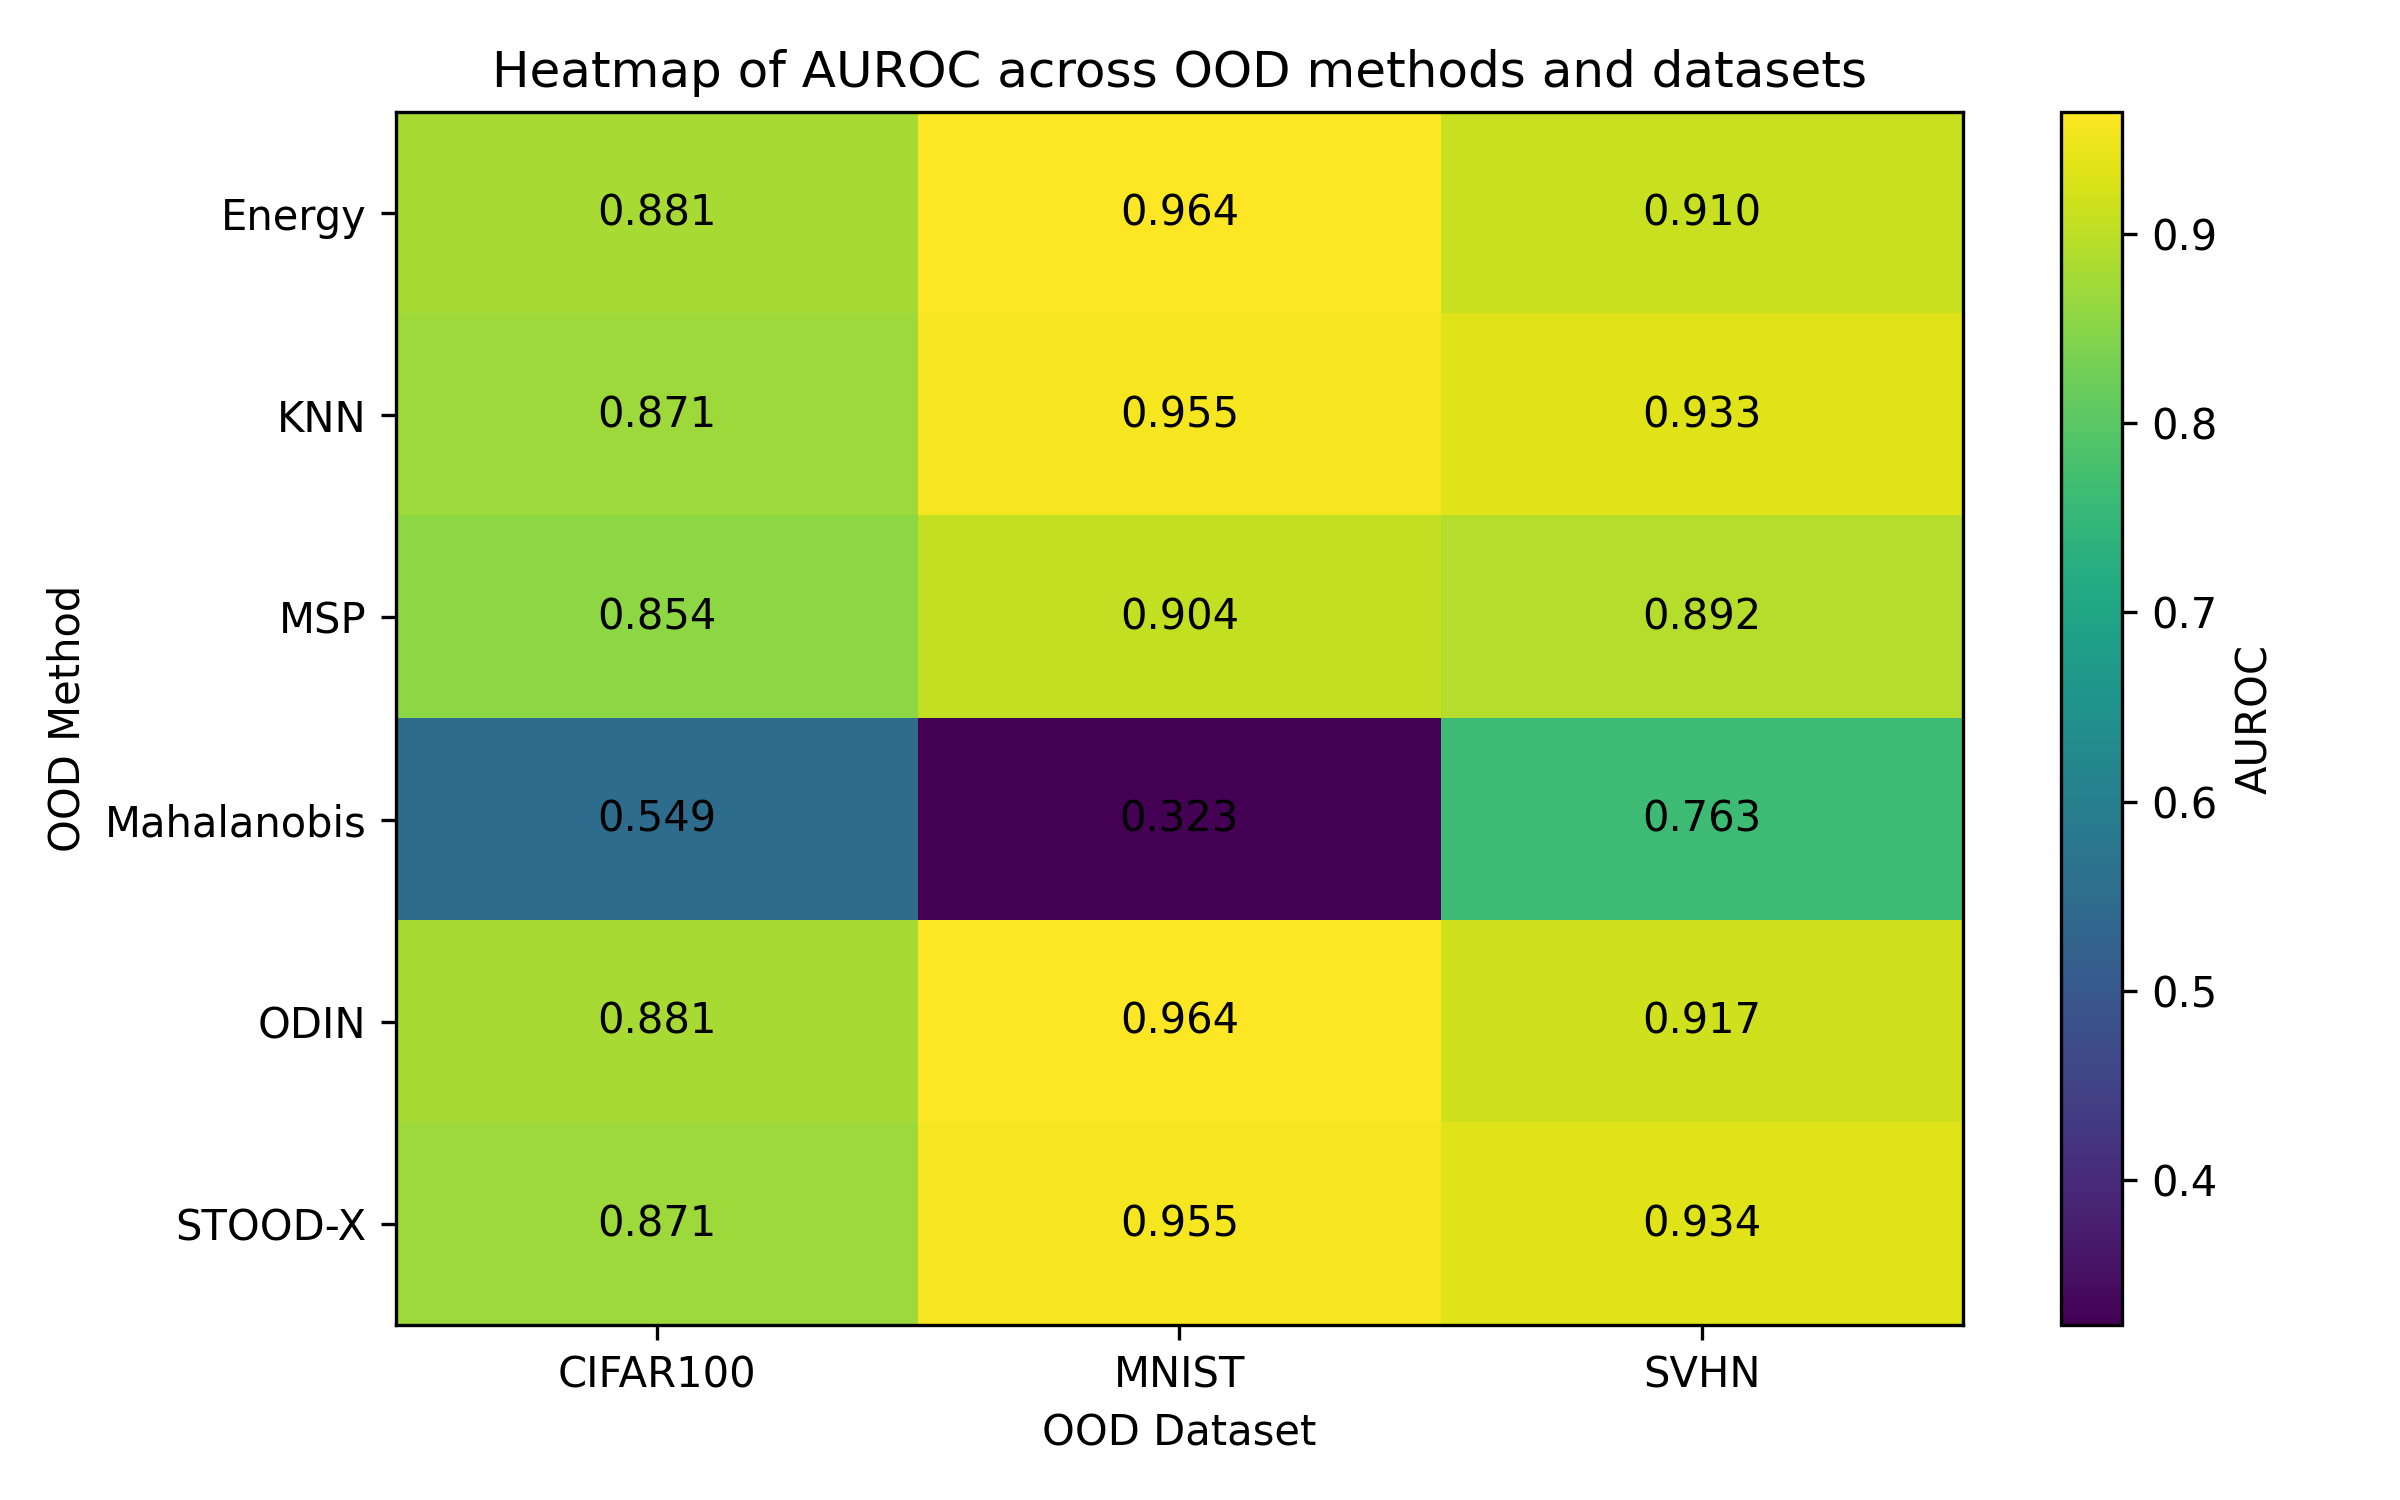
\includegraphics[width=0.49\textwidth]{heatmap_auroc_methods_datasets.png}
  \hfill
  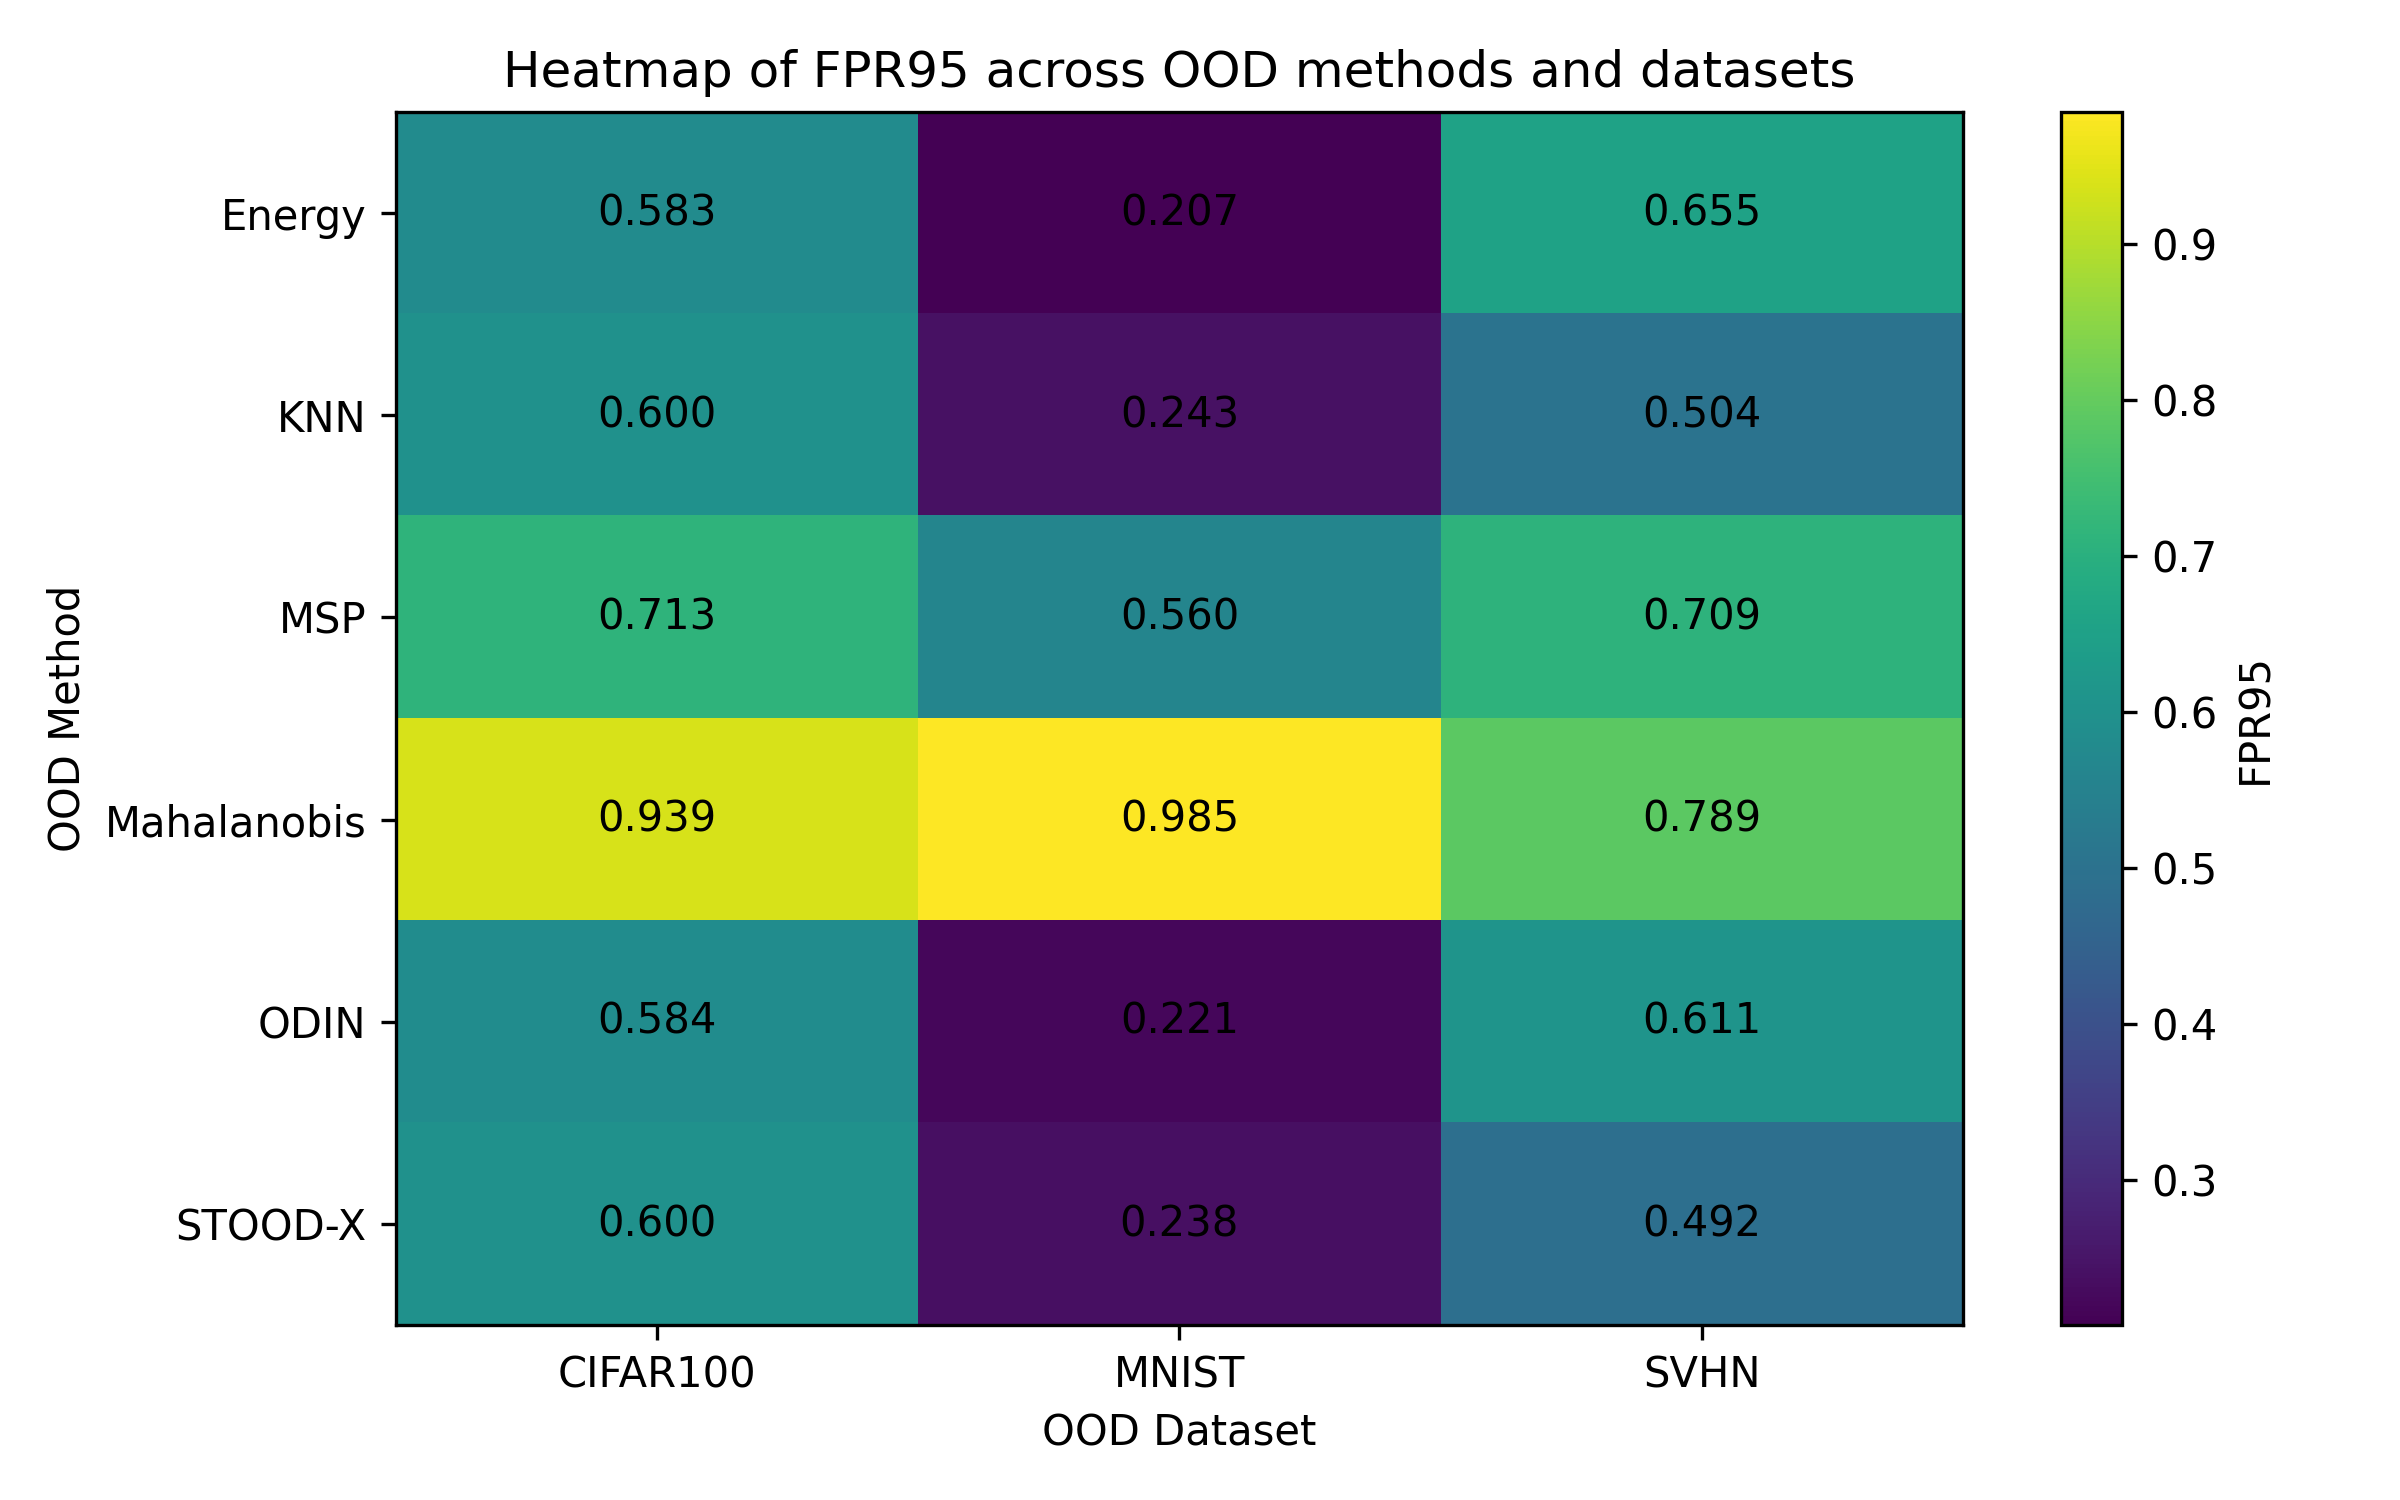
\includegraphics[width=0.49\textwidth]{heatmap_fpr95_methods_datasets.png}

  \vspace{0.8em}
  \begin{itemize}
    \item ODIN and Energy are strongest on CIFAR-100 and MNIST.
    \item KNN and simplified STOOD-X are very close, because both rely on feature-space distances.
    \item Mahalanobis underperforms, especially on MNIST and CIFAR-100.
  \end{itemize}
\end{frame}

\begin{frame}{Score and Feature-Space Evidence}
  \begin{columns}[T,onlytextwidth]
    \column{0.50\textwidth}
      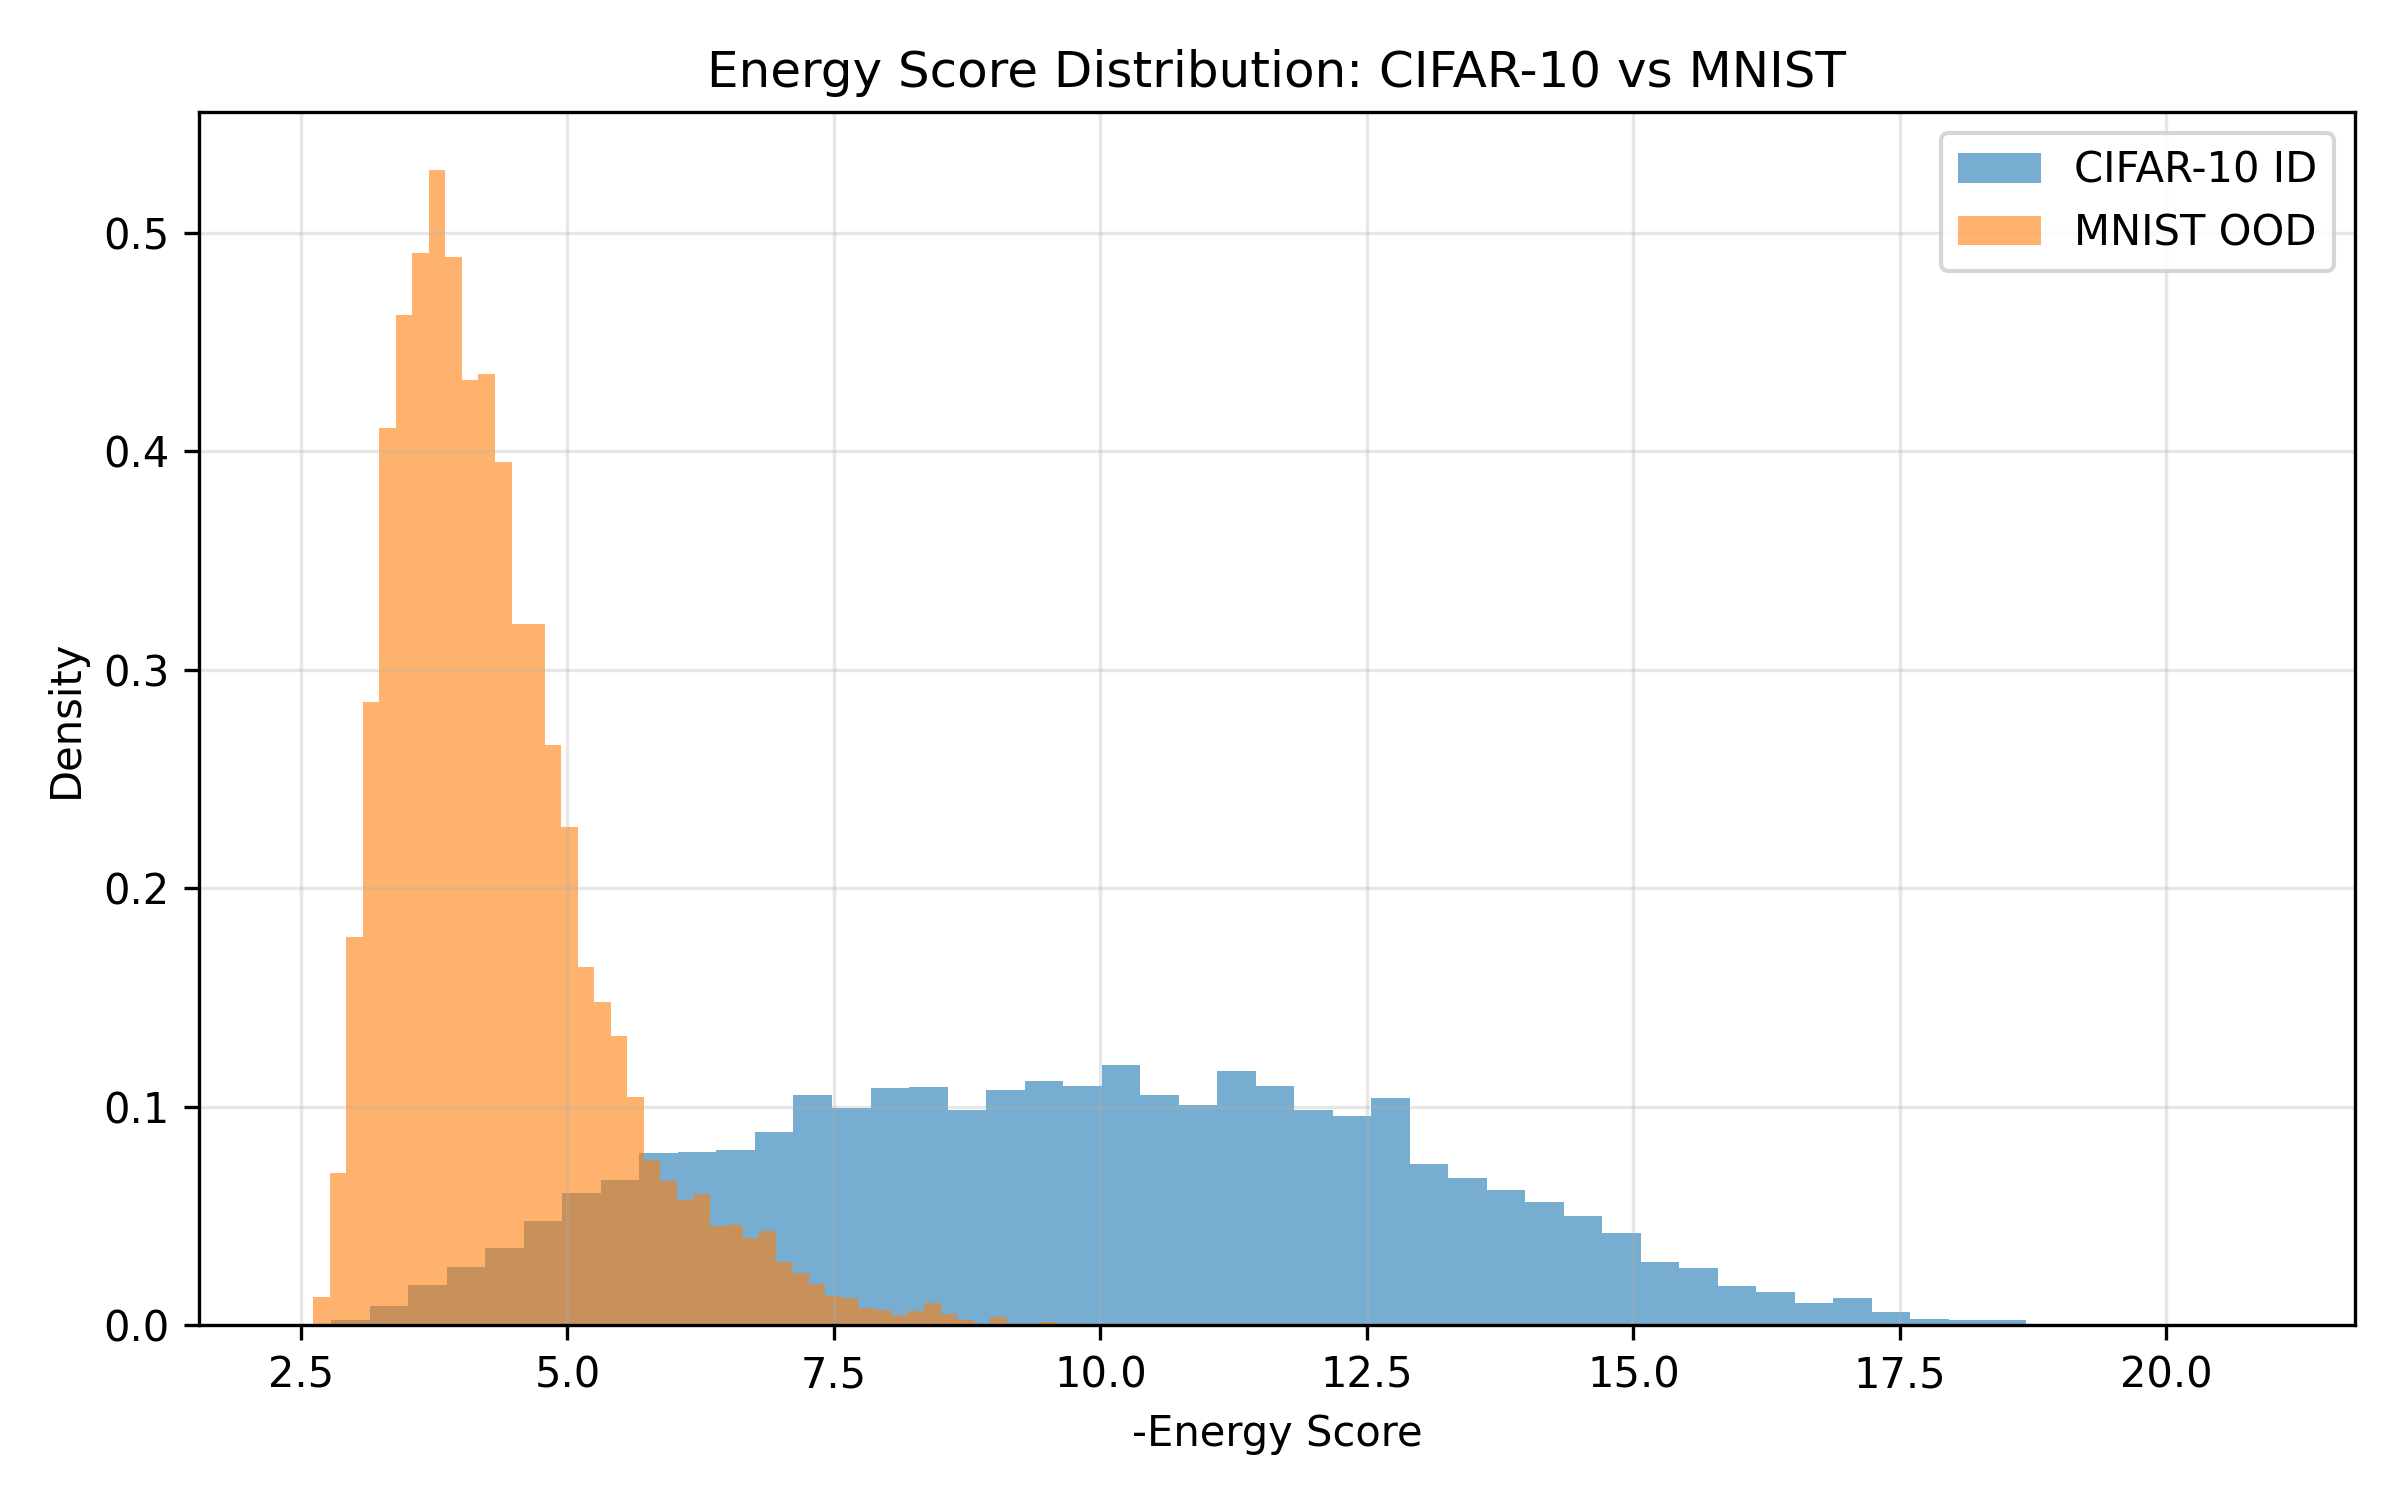
\includegraphics[width=\textwidth,height=0.31\textheight,keepaspectratio]{energy_cifar10_vs_mnist.png}
      \vspace{0.2em}

      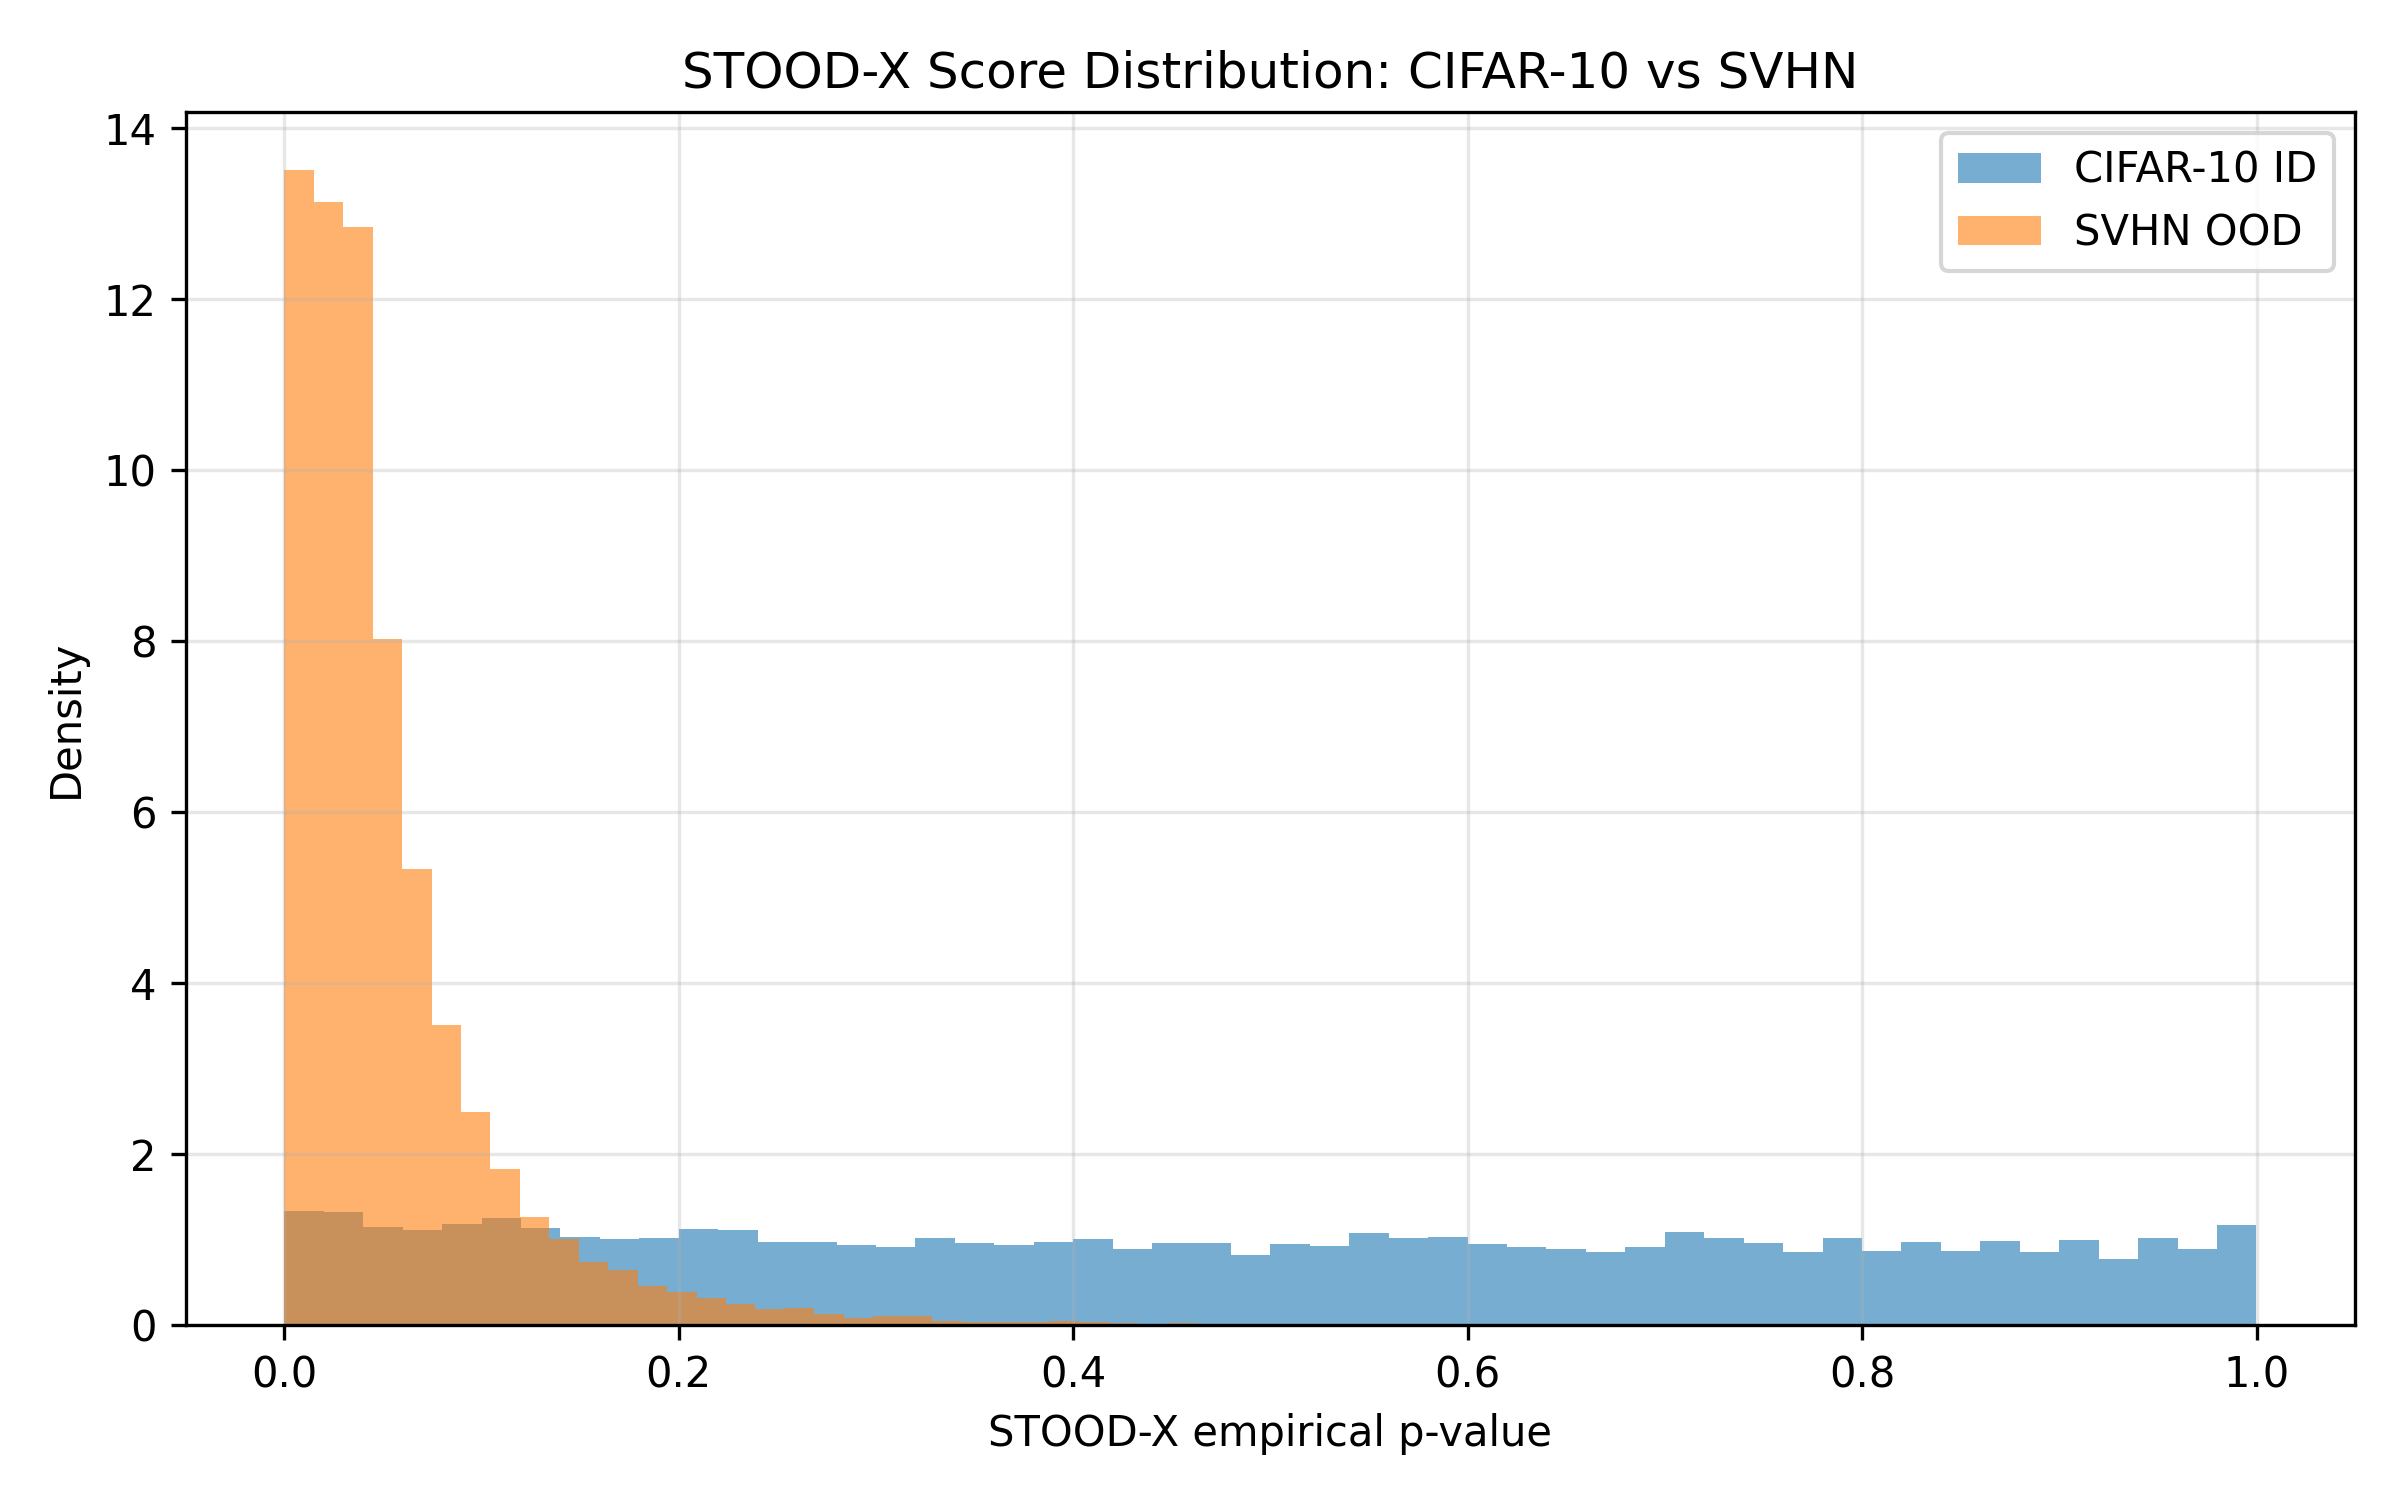
\includegraphics[width=\textwidth,height=0.31\textheight,keepaspectratio]{stoodx_cifar10_vs_svhn.png}
    \column{0.47\textwidth}
      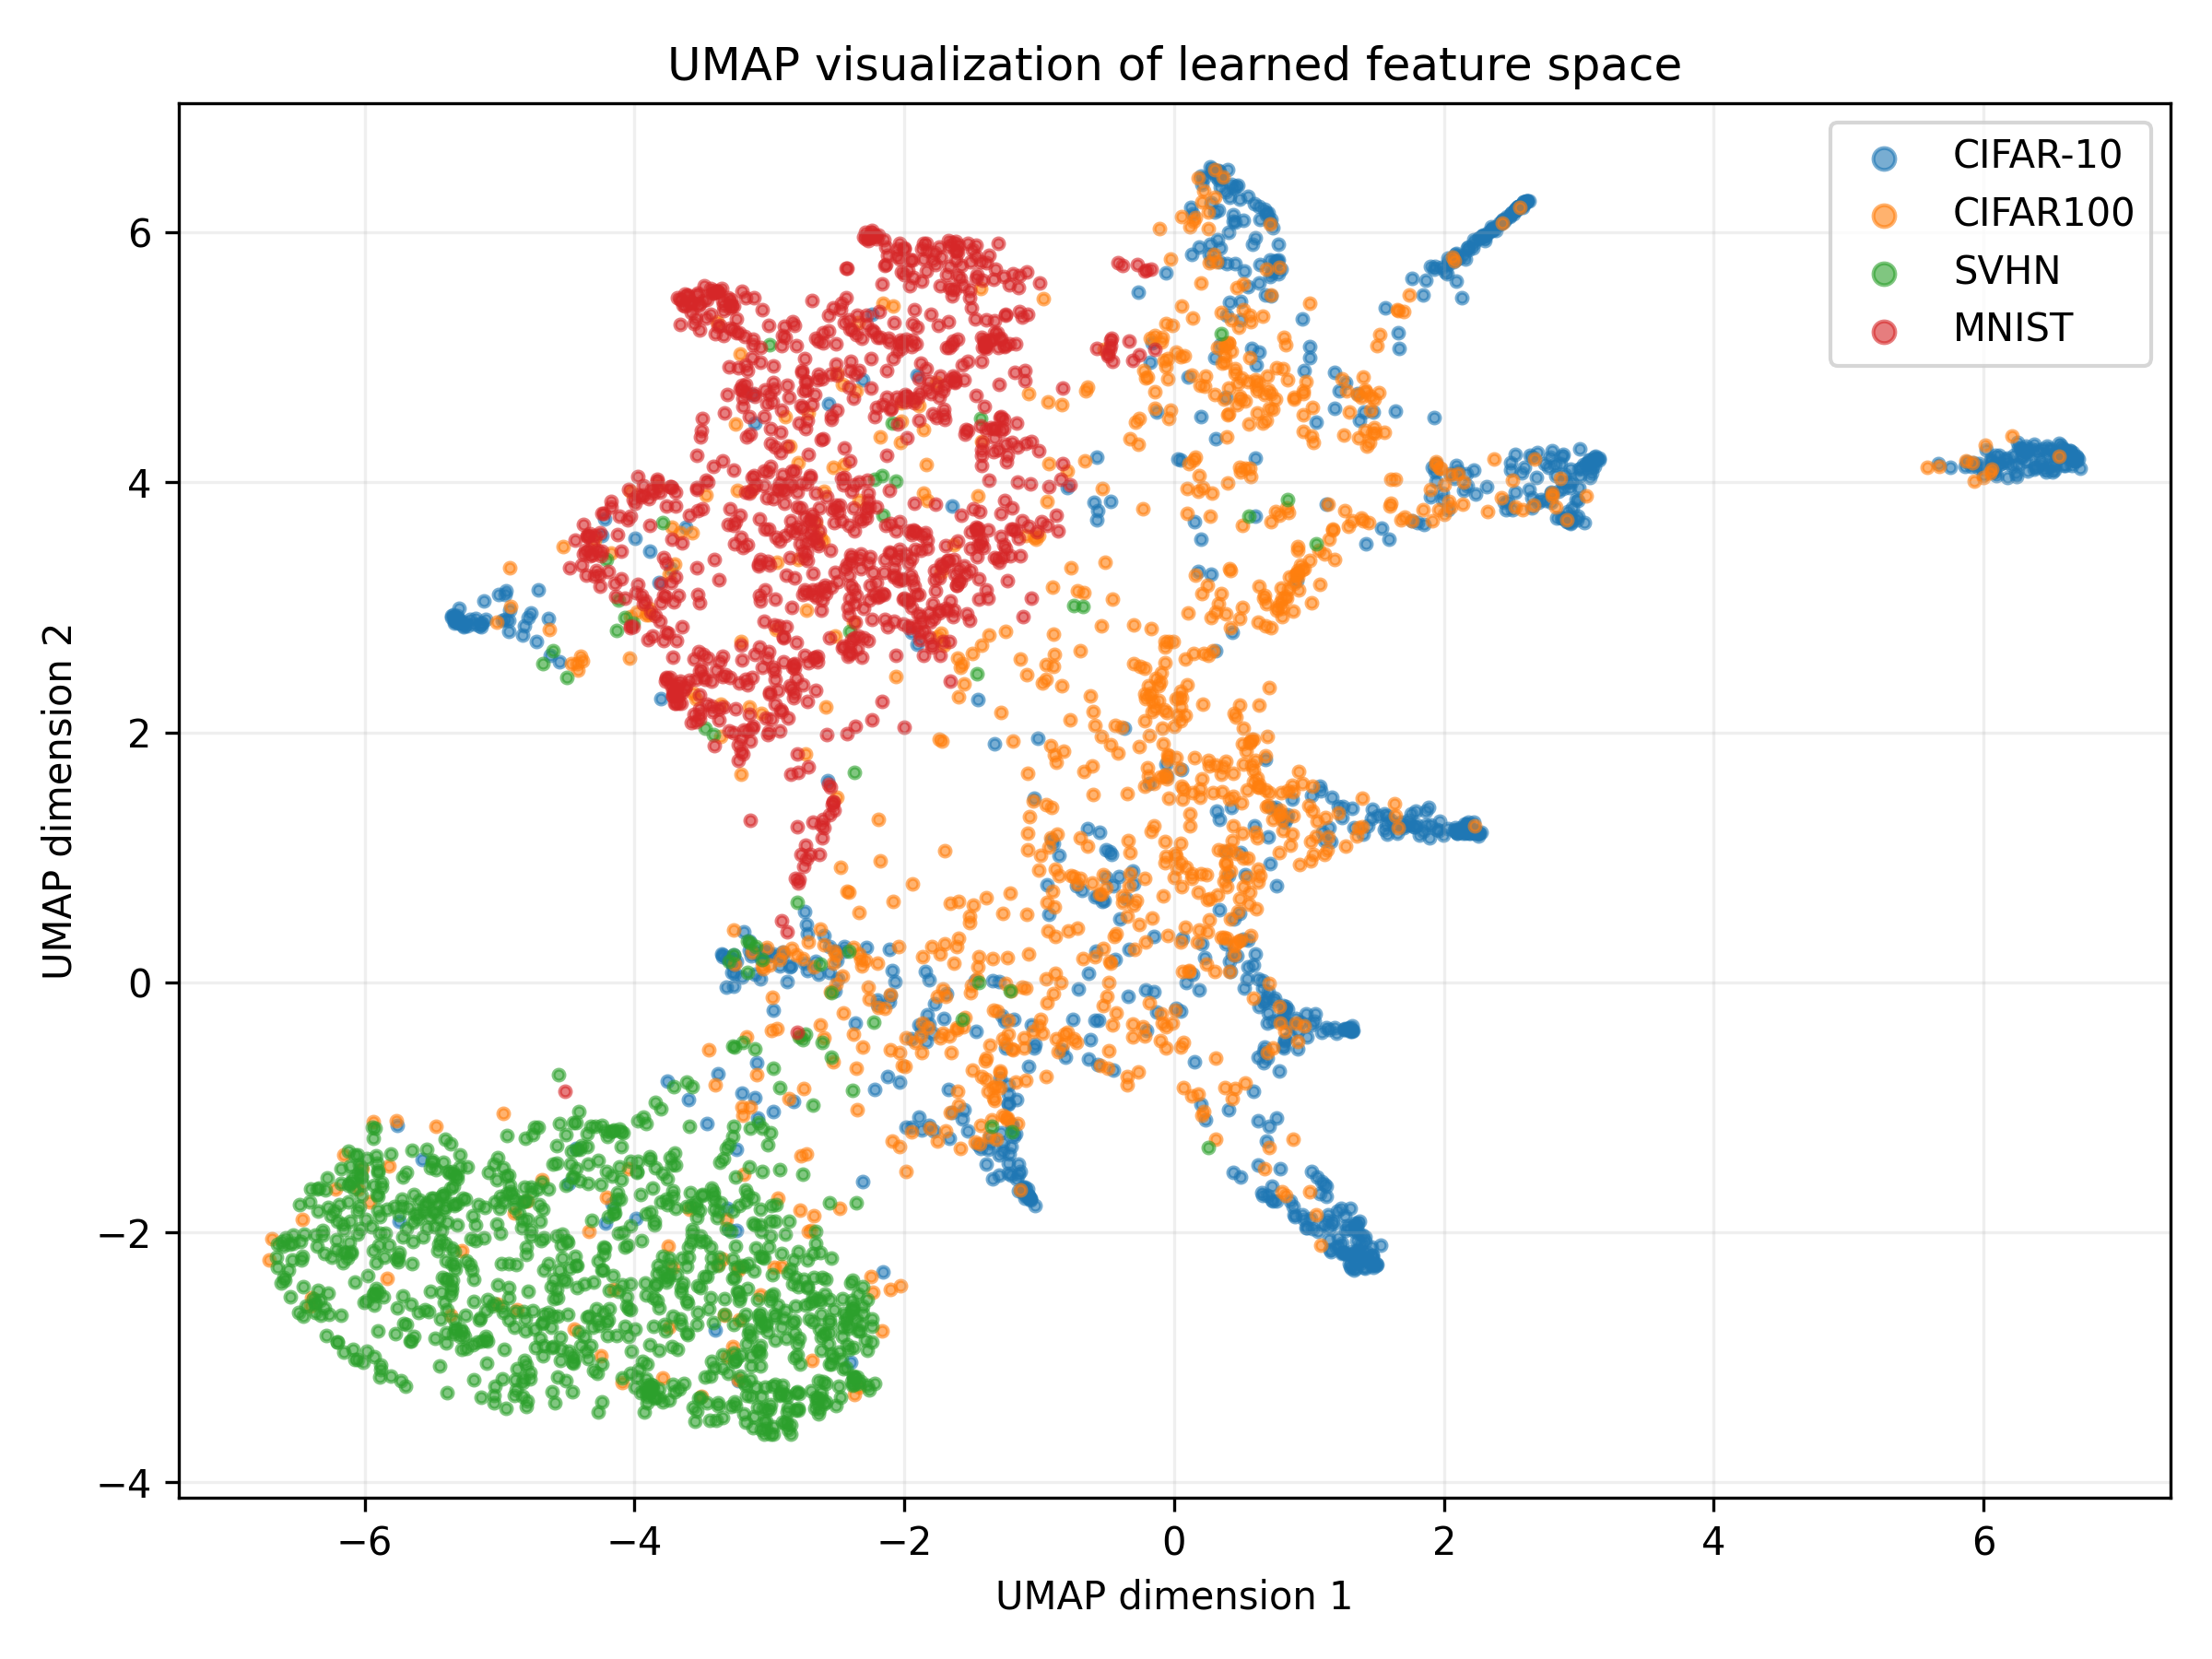
\includegraphics[width=\textwidth,height=0.52\textheight,keepaspectratio]{umap_cifar10_ood_features.png}

      \vspace{0.2em}
      \small
      \begin{itemize}
        \item Good detectors separate ID and OOD score distributions.
        \item UMAP confirms that feature geometry contains useful OOD information.
      \end{itemize}
  \end{columns}
\end{frame}

\begin{frame}{Main Conclusions}
  \begin{itemize}
    \item The ResNet-18 classifier provides a strong feature space for post-hoc OOD detection.
    \item ODIN and Energy are the best overall logit-based methods.
    \item Simplified STOOD-X is strongest on SVHN and competitive on MNIST.
    \item Feature-distance methods are useful when OOD samples are not simply low-confidence inputs.
    \item The project produces reproducible outputs: metrics tables, ROC curves, score distributions, heatmaps, t-SNE/UMAP and a final report.
  \end{itemize}

  \vspace{0.9em}
  \textbf{Limitations.} Single architecture, single training run, three OOD datasets, and only a partial STOOD-X replication.

  \vspace{0.7em}
  \centering
  \textbf{Takeaway:} OOD detection improves when classifier confidence is combined with feature-space evidence.
\end{frame}

\end{document}
